\documentclass{mpaper}
% \usepackage[bottom]{footmisc}
\usepackage{dblfnote}
\DFNalwaysdouble
\graphicspath{{./processed_data/}}
\usepackage{caption}
\usepackage{subcaption}

\begin{document}

\title{Investigating the Efficacy of QUIC for Low-Latency Streaming}
\author{Matthew Walker}
\matricnum{2310528}
\date{COMPSCI5082P (40 credits) — April 1, 2022}

\maketitle

\begin{abstract}
Until now, real-time video streaming applications have had to choose between reliable but potentially delayed transmission over TCP, or low-latency but unreliable transmission over UDP. In recent years, QUIC has emerged, which may be able to offer the best of both worlds through the use of multiple data streams. This paper evaluates three different approaches for utilising QUIC streams for real-time video streaming. The findings of this research show that by providing a stream for each RTP packet sent over a connection, QUIC is capable of providing all the features of TCP while massively reducing packet delay in lossy networks.
\end{abstract}

\section{Introduction} \label{Introduction}

\noindent The internet is becoming the primary medium for broadcasting and communications in the modern era. This shift has many advantages; Video conference calls can be made anywhere, with the only infrastructure requirement being an active internet connection. Additionally, as IPTV and Over-the-top (OTT) streaming services become widespread, consumers need no longer plan their day around programming schedules to stay up to date with the latest series. However, this transition does not come without drawbacks; The internet protocol (IP\cite{IP}) is a best-effort packet delivery service, and packets may be lost or delayed during transport.
\\\\
Due to protocol ossification in the transport layer, up until now, we have been restricted to using UDP\cite{UDP} or TCP\cite{TCP} for the transmission of real-time multimedia. Neither of these are ideal; TCP provides congestion control and ensures all data arrives intact by focusing on delivering packets reliably and in-order. However, these features can inject significant delays making TCP unsuitable for real-time media applications with strict latency bounds. For live broadcasts, this delay can be detrimental to the user experience, with consumers complaining that neighbours using more traditional receivers see events first, and spoil the outcome\cite{LIVESURVEY}. 
\\\\
On the other hand, UDP makes no effort to control the sending rate of packets, nor does it ensure that packets arrive at their destination. The simplicity of UDP introduces minimal latency, making it the protocol of choice for interactive video streaming. However, the lack of loss detection and retransmission mechanisms results in quality degradation within lossy networks. In order to improve the experience of hundreds of millions of users, a new transport protocol is required for real-time video streaming.
\\\\
QUIC is a new transport layer protocol that was initially developed by Google and has recently been published as an official internet standard by the Internet Engineering Task Force (IETF)\cite{rfc9000, rfc9001, rfc9002, gQUIC}. Unlike previous attempts to deploy new transport protocols, QUIC avoids the issue of protocol ossification by running on top of UDP, allowing QUIC packets to pass through middleboxes unobstructed. Additionally, QUIC is typically implemented in userspace, allowing modifications to be deployed with ease. Like TCP, QUIC promises ordered and reliable transmission of data. However, QUIC supports multiple ordered byte-streams, allowing it to avoid the HOL blocking\cite{HOLBlocking} issue which plagues TCP. By taking advantage of these ordered byte-streams, QUIC may reduce the delay incurred by TCP and diminish the quality degradation that can occur with UDP when used in real-time video streaming applications.
\\\\
This paper aims to answer the following questions: 
\begin{enumerate}
\item \textit{'Can QUIC provide a reduced latency compared to TCP when used to transport real-time video, without sacrificing video quality?'}
\item \textit{'Can QUIC deliver better quality real-time video than UDP, while operating within the strict latency bounds of interactive media?'}
\end{enumerate}


\noindent To answer these questions, this paper presents and evaluates three different methods for utilising QUIC streams to transmit real-time multimedia data: QUIC\_GOP utilises separate streams for each group of pictures that make up the encoded video stream; QUIC\_FPS utilises a stream for each frame in the video stream; Finally, QUIC\_PPS utilises a stream for each RTP packet that carries the encoded video stream. The performance of these QUIC implementations when used for low-latency streaming is compared to the performance of TCP, UDP and single-stream QUIC under various network conditions. To facilitate this comparison, single-stream QUIC, QUIC\_GOP, QUIC\_FPS and QUIC\_PPS were all implemented within the GStreamer\footnote{https://gstreamer.freedesktop.org/} media streaming framework.
\\\\
After covering the necessary background in Section \ref{Backgorund}, Section \ref{Design Rationale} discusses the rationale behind the design of \newline QUIC\_GOP, QUIC\_FPS and QUIC\_PPS. Section \ref{Implementation} covers the implementation of the QUIC-GStreamer elements, the GStreamer pipeline used for testing, and the test framework used during evaluation. Section \ref{Results} examines the results of the evaluation and their significance. Section \ref{Related Work} reviews related work. Section \ref{Conclusions} presents the conclusions of the paper. Finally, section \ref{Future Work} discusses the limitations of this research and the potential avenues for future work.


\section{Background} \label{Backgorund}

\noindent In this section, the paper discusses the different features of ordered, reliable, congestion-controlled transport protocols that can introduce delay when transmitting real-time video data. However, before this, the paper first describes a key component of real-time multimedia transmission: The Real-time transport protocol.

\subsection{Real-time Transport Protocol} \label{Real-time Transport Protocol}

\noindent The Real-time transport protocol (RTP) is an application layer protocol designed to support applications in the transmission of real-time multimedia data\cite{RTP}. A key feature of RTP is the sequence numbering of packets; While RTP does not make any effort to ensure reliable, ordered delivery of packets, its sequence numbers allow applications to correct the ordering of packets. An example of this is a jitter buffer, which will delay out-of-order packets until preceding packets arrive so that they can be provided to the rest of the application in the correct order. Another important feature of RTP is its timestamping. RTP timestamps can inform the client of the appropriate time to decode and present multimedia data. Additionally, timestamps can be used to synchronise separate data streams, such as audio and video.
\\\\
As well as providing timestamping and sequence numbers, RTP also supports the creation of payload format specifications. These specifications define how specific media types are packaged into RTP packets. This allows RTP to be used with a wide range of media types, making the protocol easily extensible when new media types become available. 


\subsection{Congestion Control} \label{Congestion Control}

\noindent Congestion Control algorithms are used by TCP and QUIC to maximise network link utilisation and avoid the loss of packets due to network congestion. These algorithms focus on maximising throughput rather than minimising packet latency and, as a result, can inject delays that are unideal for real-time video streaming. With this in mind, it is essential to select a congestion control algorithm that introduces as little latency as possible.
\\\\
There are many congestion control algorithms available, but currently, the majority of QUIC implementations provide only CUBIC\cite{CUBIC} and BBR\cite{BBR} as options. Due to this, the paper will only discuss CUBIC and BBR.
\\\\
CUBIC is a loss-based congestion control algorithm. It increases its congestion window until the router buffer at the bottleneck link fills and begins to drop packets. When this loss is detected, CUBIC decreases its congestion window, resulting in a decreased sending rate. This model has two major issues when it comes to real-time multimedia: 

\begin{enumerate}
\item Congestion is only detected when the buffer for the bottleneck link becomes full, at which point the sending rate drops and the buffers drain. As a result, the buffers are at least partially filled for a significant percentage of the connection. When buffer queues are not empty, the time taken for a new packet to work its way through the queue adds to the overall packet delay. This phenomenon is known as "bufferbloat".
\item As loss is used as the indicator of congestion, any other sources of packet loss, such as signal interference on a wireless network, will result in the sending rate dropping. This will also significantly contribute to packet delay.
\end{enumerate}

\noindent BBR takes a different approach; A model of the network's round-trip time (RTT) and bottleneck bandwidth is updated with each packet acknowledgement. BBR uses this model to pace packets such that the full bottleneck link capacity is utilised without filling the router buffer. This eliminates the delay caused by "bufferbloat". While BBR might seem ideal for real-time multimedia, it does have a drawback: When the estimated RTT has not decreased in the last 10 seconds, BBR will enter a PROBERTT state for at least 200ms. When in this state, the congestion window drops to the size of 4 packets, allowing any packets in router buffers to drain. This allows BBR to update its estimated RTT, but the drop in sending rate may impact the timely delivery of real-time multimedia data. Additionally, while BBR does not use loss as an indicator of congestion, it does respond to loss events by entering 'loss recovery'. BBR will lower its sending rate in response to loss, temporarily reducing the congestion window to be equal to the number of packets currently in flight. Still, the impact of PROBERTT and BBR's loss response is significantly less than that of CUBIC's issues on high loss networks. 


\subsection{Flow Control} \label{Flow Control}

\noindent While Congestion Control concerns itself with the buffers of routers in the network, Flow control modulates the sending rate of TCP and QUIC based on the advertised capacity of the client. TCP receivers will inform senders of their current receive buffer availability using the window size of the TCP segment header. If a window size of 0 is received, the TCP sender must stop sending altogether. QUIC is slightly more complicated as it maintains flow control limits for both individual streams and connections as a whole. When a per-connection or per-stream flow control limit is reached, the server is unable to transmit any more data until the receiver provides additional flow control credit. These restrictions introduce a delay that impacts the timely delivery of packets.
\\\\
Within QUIC, there are two possible strategies for increasing flow control limits. The first is for the receiver to wait until the sender sends a DATA\_BLOCKED or \newline STREAM\_DATA\_BLOCKED frame. At which point, the receiver will provide additional flow control credit by sending a MAX\_DATA or MAX\_STREAM\_DATA frame. In this case, the sender will be unable to transmit new data until at least 1 RTT has passed. The resulting delay could cause any waiting RTP packets to be delivered after their playback deadline.
\\\\
The second strategy requires the receiver to monitor the amount of data received and update its flow control limits prior to the limit being reached. If successful, QUIC's flow control limits should have no impact on the delay. However, the nature of real-time video streaming means that data will usually arrive in bursts, and the transmission of a single I-frame could easily reach low flow control limits. To avoid any delays, it will be necessary for the flow control limits to be at least as large as the amount of data the sender will send within a single RTT. This will allow enough time for the receiver to provide additional flow control credit before the existing limits are reached.


\subsection{Head-Of-Line Blocking} \label{Head-Of-Line Blocking}

\noindent Reliable protocols such as TCP, that promise to deliver data in order, will prevent data that has arrived at the client from being delivered to the application until all earlier data in the stream has arrived. This is known as head-of-line (HOL) blocking. For some applications, this simply wastes time that could be spent processing the data that has already arrived. For real-time media applications, HOL blocking is much more problematic; By the time lost data is retransmitted, the playback deadline could already have passed. HOL blocking can cause a knock-on effect, where the subsequent packets will be made available to the application too late, despite arriving on time.
\\\\
When working with a single stream, the blocking time for a missing packet is equivalent to the time taken to retransmit the missing packet. TCP considers a packet lost when it receives three duplicate acknowledgements. Similarly, in QUIC, if a packet with packet number $K$ has not received an acknowledgement, it will be considered lost when a packet with a packet number greater than or equal to $K+3$ is acknowledged. Assuming there is a consistent spacing between packets, $T_{spacing}$, then the minimum retransmission time for a missing packet, $T_{retx}$ is:

\[ T_{retx} = (3*T_{spacing}) + RTT  (1)\] 

\noindent The above equation is a lower bound on the retransmission time; If any subsequent packets are lost, or the acknowledgements of those packets are lost, then the retransmission time, and therefore the HOL blocking time, for a missing packet will be greater. 
\\\\
Regarding $T_{spacing}$, the worst-case scenario for real-time multimedia is that each frame is smaller than the path MTU. In this case, each frame can be carried by a single ack-eliciting packet, and so $T_{spacing}$ would be equal to the duration of each frame. For 24fps video, this would impose a minimum retransmission delay of roughly 126ms. However, for the majority of video streaming, the encoded video frames will be too large to fit within a single RTP packet. As a result, depending on the position of the lost packet within the frame, there are two possible lower bounds on retransmission time:
\\\\
Let $T_{intra\_frame\_spacing}$ be the spacing between packets carrying the same frame and $T_{inter\_frame\_spacing}$ be the spacing between the last packet in one frame and the first packet in the next. We would expect $T_{intra_frame_spacing}$ to be close to $0$ as all of the frame data should be sent immediately. $T_{inter_frame_spacing}$ would be determined by the capture rate. In the case that there are at least three packets carrying the same frame transmitted after a lost packet, the minimum retransmission will be:

\[ T_{retx} = (3*T_{intra\_frame\_spacing}) + RTT  (2)\]

In the case that the missing packet is one of the last three packets carrying a frame, the minimum retransmission will be:

\[ T_{retx} = (2*T_{intra\_frame\_spacing}) + T_{inter\_frame\_spacing} + RTT (3)\]

QUIC is capable of utilising multiple streams within a single connection. HOL blocking exists within individual streams, but streams are independent of one another. So, if a loss occurs on one stream, the others can proceed unaffected and continue to deliver data to the application. Thus, when used correctly, QUIC's streams should be able to minimise the delay induced by HOL blocking. In the following subsection, the paper discusses the three levels of abstraction in an H264 encoded video stream, which provides insight into how QUIC streams can be best utilised.


\subsection{The Structure of Encoded Video} \label{The Structure of Encoded Video}

\noindent Raw video frames are massive in terms of bytes. Their size makes storage and transmission of raw video infeasible, and so compression is employed to reduce their size. Compressed video frames can be broken into three categories: I-frames, also known as key-frames, are compressed using spatial redundancy alone, allowing them to be decoded independently; P-frames, or predicted frames, only encode the changes compared to previous frames, allowing a much greater reduction in size but preventing them from being decoded independently; B-frames, or bi-directional frames, are similar to P-frames but rely on references to both previous and subsequent frames.
\\\\
As the encoder requires knowledge of future frames to produce B-frames, these are not suitable for low-latency real-time multimedia where the goal is to transmit frames as soon as possible. For this reason, this paper will only consider I-frames and P-frames.
\\\\
At the highest level of abstraction, I-frames and P-frames can be viewed as structures called "Group of Pictures" \newline (GOPs). A GOPs starts with an I-frame followed by all the subsequent P-frames before the next I-frame in the encoded video. In this way, a GOPs represents a collection of frames with interdependencies only with other frames within the GOPs. Thus, GOPs can be considered independently decodable units.
\\\\
Depending on the codec used, there may be a lower level of abstraction than frames. NAL units in the H264 video encoding standard are an example of this. H264 is currently the most popular encoding standard amongst industry developers\footnote{https://go.bitmovin.com/video-developer-report-2019} and is used for both live broadcasting\footnote{https://www.streamingmediablog.com/2017/05/hulus-live-streaming-workflow.html} and video conferencing. This makes H264 an appropriate codec choice for the research conducted in this paper. As mentioned, H264 utilises Network Abstraction Layer (NAL) \newline units. NAL units format the encoded video data into a more appropriate form for transmission over a network, making it easy to use H264 in conjunction with protocols such as RTP. NAL units are grouped in "Access" units, with a complete unit representing a frame in the encoded video. Access units often contain redundant NAL units allowing the decoder to recover from NAL unit loss.

\section{Design Rationale} \label{Design Rationale}

\noindent Three different methods of utilising QUIC's streams to avoid HOL blocking were devised. All streams are reliable, and all missing data will be retransmitted. The original intention was also to add deadline awareness at the server to prevent the retransmission of packets that will not arrive in time to be useful. However, due to time constraints, this feature has not been added. Provided that there is sufficient bandwidth in the network, the overhead of retransmitting 'stale' packets should be negligible.
\\\\
The first method, "QUIC\_GOP", creates a new QUIC stream for every Group of Pictures in the encoded video. This method has the least overhead in terms of streams created and managed by the QUIC implementation. This method removes any HOL blocking between GOPs, and initially, it seems sensible to perform HOL blocking within GOPs. After all, the P-frames in a GOP would be useless if the preceding I-frame has not arrived. However, the scenario where a P-frame is lost must also be considered. In this case, a missing P-frame would temporarily prevent subsequent frames from being delivered to the application, potentially causing them to be delivered after their playback deadline. Research has shown that missing P-frames do not necessarily impact the user experience, as subsequent P-frames can allow the picture to recover\cite{FrameRecovery}. With this being the case, if the overhead of creating many streams is negligible, it is anticipated that QUIC\_GOP will be less successful than the other methods presented in this paper.
\\\\
The second method, "QUIC\_FPS", creates a new QUIC stream for every frame in the encoded video. This method represents a middle ground between QUIC\_GOP and the final method in terms of stream overhead. If a P-frame is lost, subsequent P-frames will not be blocked and can be passed to the decoder. QUIC\_FPS does not provide any benefit if an I-frame is lost but does avoid the P-frame HOL blocking issue that QUIC\_GOP experiences.
\\\\
The final method, "QUIC\_PPS", creates a new QUIC stream for every RTP packet required to transmit the stream. This method represents an extreme for stream overhead. Splitting data into smaller units does not provide any benefits in terms of HOL blocking compared to using a NAL unit per stream, as anything smaller than a NAL unit would not be useful to the application. However, using an RTP packet per stream improves the utility of QUIC\_PPS for other forms of real-time media, such as audio. As mentioned in section \ref{The Structure of Encoded Video}, H264 will place redundant NAL units in each Access unit. As QUIC\_FPS is still capable of suffering from HOL blocking within frames/Access units, redundant NAL units may prevent subsequent, useful NAL units from being delivered. QUIC\_PPS does not have this issue; if a NAL unit has not arrived before the deadline for its frame, then QUIC\_PPS will not block NAL units for that frame that have arrived from being be passed to the application. If the missing NAL unit was redundant, then QUIC\_PPS should be able to deliver a frame where QUIC\_FPS would not.
\\\\
In essence, the three methods represent a tradeoff between the potential for HOL blocking and the overhead for creating and managing streams. However, given the processing requirements for encoding and decoding video, it is anticipated that the overhead of creating many streams will be negligible in comparison.
\\\\
A final point of consideration is message framing. The streams used by QUIC\_GOP, QUIC\_FPS and QUIC\_PPS naturally frame GOPs, frames and RTP packets, respectively. However, this is only true if the implementation waits until all data has arrived on a stream before passing data to the application. This strategy is problematic for QUIC\_GOP; GOPs can range in size from a few hundred milliseconds to multiple seconds, depending on the interval between I-frames. If no data is passed to the application until the entire GOP has arrived, then the initial frames will be significantly delayed. This issue also has a minor impact on QUIC\_FPS; Consider a hypothetical frame split into 8 NAL units for transport. If the first 7 NAL units arrive, but the 8th is lost, then the first 7 NAL units will not be made available to the application until the 8th is retransmitted. If the 8th NAL unit was redundant, this strategy might prevent useful data from being passed to the application before the playback deadline.
\\\\
To avoid this issue, at the client-side, QUIC\_GOP and \newline QUIC\_FPS must provide data to the application before the stream is finished. However, passing incomplete RTP packets to the application may cause issues, so another form of message framing must be applied. RFC4571\cite{RFC4571} describes a method for framing RTP packets for use with TCP; A two-byte length field is appended to the beginning of each packet before sending, allowing the packets to be parsed by the client application. Nothing about this method is specific to TCP, so it can be easily applied to QUIC\_GOP and QUIC\_FPS.
\\\\
\section{Implementation} \label{Implementation}

Comparison of QUIC\_GOP, QUIC\_FPS and QUIC\_PPS to TCP, single-stream QUIC and UDP, required the development of three pieces of software: GStreamer pipelines that could simulate the functionality of a real-time video streaming application; GStreamer element implementations for single-stream QUIC and QUIC\_GOP, QUIC\_FPS, \newline QUIC\_PPS; And a test framework that could construct the pipelines and evaluate each implementation under various network conditions. This section of the paper discusses the implementation of this software.

\subsection{GStreamer Pipelines} \label{GStreamer Pipelines}

\noindent To model a real-time multimedia streaming application, \newline GStreamer pipelines were designed that carry out most of the steps these applications perform. The only steps not carried out are capture and rendering, as the pipelines do not have access to the necessary devices from within the network simulation. These processes would add to the total application delay, and this will need to be taken into account during the analysis of the test results.
\\\\
The server-side pipeline (Figure \ref{fig:GST_Server}) reads raw video data from a file and parses the frames; these frames are then passed to the H264 encoder every 41.666667ms to simulate capture at a rate of 24 fps. The encoded data is then passed to the RTP payloader, which places the NAL units that make up the frame into RTP packets. If the network element at the end of the server-side pipeline does not provide framing for the RTP packets, as is the case with TCP, single-stream QUIC, QUIC\_GOP and QUIC\_FPS, then an RTP stream payloader is added to the pipeline in order to append the length of each packet as per RFC 4571\cite{RFC4571}. Finally, data is passed to the network element for transmission. 
\\\\
The test video used for all experiments is a 60-second clip of the Big Buck Bunny animation\footnote{http://commondatastorage.googleapis.com/gtv-videos-bucket/sample/BigBuckBunny.mp4} that has been decoded into raw video data. A video resolution of 720p was selected as it matches the resolution used by video conferencing applications such as Zoom and is also a common resolution used for live broadcasts. When the pipeline encodes the data, the resulting frames are too large to be carried in a single RTP packet. Thus, the possible lower bounds on retransmission time for a lost packet are given by equations (2) and (3) from section \ref{Head-Of-Line Blocking}.
\\\\
The client-side pipeline (Figure \ref{fig:GST_Client}) receives data over the network using one of the network elements described above. If the network element does not provide framing, buffers are passed to the RTP stream depayloader, which extracts RTP packets from the stream of data. The RTP packets are then passed to an RTP jitter buffer that corrects the ordering of packets and will hold packets up to a specified delay to give time for missing packets to arrive. RTP packets are then depayloaded, and the NAL units carried within are passed to the decoder. Finally, as rendering was not possible, the frames are passed to a fakesink element which simply discards the data.

\begin{figure}
  \begin{center}
  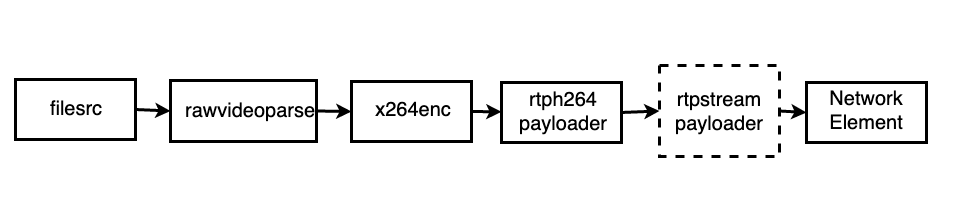
\includegraphics[scale=0.25]{Server-side_pipeline.png}
  \end{center}
  
  \caption{\label{fig:GST_Server}Server-side Gstreamer pipeline. For clarity, this diagram leaves out a modified identity element that enforces the 24fps frame delivery rate.}
\end{figure}

\begin{figure}
  \begin{center}
  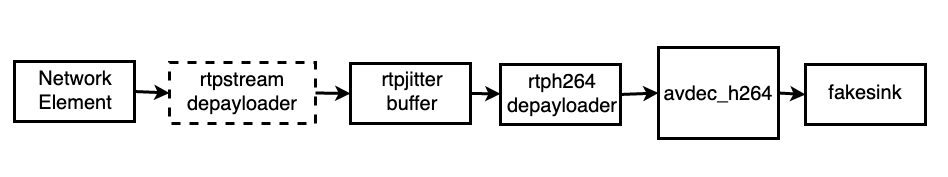
\includegraphics[scale=0.25]{Client-side_pipeline.png}
  \end{center}
  
  \caption{\label{fig:GST_Client}Client-side GStreamer pipeline}
\end{figure}

\subsection{Network Elements} \label{Network Elements}

\subsubsection{UDP and TCP} \label{UDP and TCP}

\noindent TCP and UDP element plugins for GStreamer already exist, and the plan was to utilise these elements during testing.  Initial experimentation showed no issues with the udpsink and udpsrc\footnote{https://gstreamer.freedesktop.org/documentation/udp/} elements, so these were used to evaluate UDP. However, the initial experimentation with the TCP elements showed severe flaws. The cause was unclear, but most of the RTP packets did not arrive intact, and no frames were successfully decoded.
\\\\
As the existing TCP elements were clearly unviable, new TCP element plugins were developed. The server-side sink element, tcpsink, will bind a socket to the given address and port, and wait to receive a connection. Once a connection has been established, whenever tcpsink receives a buffer from upstream, it will write all data within the buffer to the socket. tcpsrc is similarly simple; tcpsrc connects to the given port and address, reading any available data from the connection when a buffer is requested.
\\\\
As TCP utilises congestion control, a decision had to be made about which algorithm to use. TCP has many congestion control algorithms to choose from, but the QUIC implementation used by the QUIC element plugins provides only two choices: BBR and CUBIC. For fairness, it was important that the TCP and QUIC elements used the same algorithm. For the reasons described in section \ref{Congestion Control}, BBR was chosen as the congestion control algorithm.
\\\\
Finally, some additional design decisions were made to reduce latency as much as possible. The TCP\_NODELAY socket option was set, disabling Nagle's algorithm to ensure that packets are sent as soon as data is written to the socket. TCP\_QUICKACK was also enabled, causing acknowledgements to be sent as soon as possible to allow lost packets to be detected and retransmitted earlier. During initial testing, the default TCP receive buffer size (87380 bytes) was found to be sufficiently large such that no delays would be introduced due to flow control.

\subsubsection{QUIC} \label{QUIC}

\noindent Despite being standardised only recently, QUIC has a number of actively developed implementations to choose from. The LSQUIC\footnote{https://lsquic.readthedocs.io/en/latest/} library was chosen as it is simple to install, has a clear API with excellent documentation, examples and tutorials, and supports all QUIC features and extensions. Within LSQUIC, an engine instance handles connection establishment and manages active connections. The application reads messages from a datagram socket, passing them to the engine, which identifies the associated connection, decrypts and processes the QUIC packets, and returns encrypted QUIC packets to be sent in response. LSQUIC was used to create GStreamer element pairs for the QUIC\_GOP, QUIC\_FPS and QUIC\_PPS stream creation methods described in section \ref{Design Rationale}. For comparison, an element pair was also created for single-stream QUIC (This will be referred to as QUIC\_SS). 
\\\\
Any delays in acknowledgement could cause delayed retransmission, so delayed acknowledgements were disabled. It was also desirable to have LSQUIC send packets as soon as data is written to a stream, similar to the TCP\_NODELAY option. However, LSQUIC does not provide this functionality, so the source code was modified to prevent the buffering of data before sending. The delay\_onclose option was enabled to prevent any connections from being closed while there are still unacknowledged packets or outstanding retransmissions. Once again, for the reasons described in section \ref{Congestion Control}, BBR was selected as the congestion control algorithm.
\\\\
As noted in section \ref{Flow Control}, a potential source of delay is QUIC's connection flow control and stream flow control. On the client-side, LSQUIC will monitor the amount of data received in each stream and across the connection as a whole. When the amount of data received reaches half of the flow control limit, the limit is raised, and a MAX\_DATA (for connection-level flow control) or MAX\_STREAM\_DATA (for stream-level flow control) is transmitted to the server. Unfortunately, LSQUIC's default initial flow control limits were small enough that they would frequently be reached at the server-side before a MAX\_STREAM\_DATA or MAX\_DATA frame arrived. To combat this, the initial flow control values were raised on the client-side such that the limit would not be reached at the server-side. The necessary starting values varied depending on the RTT and were identified via experimentation. This strategy worked well for the purpose of this research but would not be viable in practice. This limitation will be further discussed in section \ref{Future Work}.
\\\\
Early experimentation showed a few issues with using \newline LSQUIC to implement QUIC\_PPS. Firstly, using a stream per RTP packet results in the number of streams growing incredibly quickly. This growth can lead to the default maximum number of active streams being reached repeatedly, leading to delays in creating new streams. The maximum allowed active streams for a connection was increased to avoid this issue. Secondly, LSQUIC will try to place data from multiple streams into a single packet when possible to improve transmission efficiency. This is allowed as per the QUIC specification\cite{rfc9000}. However, as mentioned in the specification, this can lead to the loss of a single QUIC packet impacting multiple streams, which is undesirable when trying to eliminate any form of HOL blocking. This functionality was disabled by modifying the source code such that every packet had an associated stream, preventing frames from multiple streams from being placed in the same QUIC packet. Lastly, a potential bug was discovered within LSQUIC; When new streams are created, data written to these streams will be sent even if there is no space left in the current congestion window. Packets queued for retransmission are not sent until the congestion window allows, potentially creating a delay before retransmission occurs as the amount of unacknowledged data in flight will not decrease. To prevent these retransmission delays, extra checks were added to ensure that packets were not sent until the congestion control algorithm allowed.


\subsection{Test Framework} \label{Test Framework}
\noindent To evaluate each network element, a test framework was created using Python\footnote{https://www.python.org/}. The test framework loads test parameters and the descriptions of the pipelines containing the network elements to be tested from configuration files. The performance of each network protocol implementation when used to transmit real-time video data was evaluated under various network conditions.

\subsubsection{Test Parameters} \label{Test Parameters}
\noindent The following parameters varied between tests:

\begin{itemize}
  \item Propagation Delay: The time taken for a packet to traverse the network. Values of 10, 30, 50, 100 and 150 milliseconds were used during testing. These values are a combination of the experiment values recommended in RFC 8868\cite{RFC8868} and latency values reported in a 2018 Ofcom report\cite{OFCOM}.
  \item Packet Loss: The chance of a packet being lost during transit. Values of 0\%, 0.1\%, 1\%, 5\%, 10\% were used during testing. These values are a combination of the experiment values recommended in RFC 8868\cite{RFC8868} and latency values reported in a 2018 Ofcom report\cite{OFCOM}.
  \item Buffer Delay: The maximum amount of time a packet will be held in the jitter buffer while waiting for lost or reordered packets. Values 42, 84, 126, and 168 were chosen. These values represent a buffer of 1, 2, 3 and 4 frames at 24 fps.
\end{itemize}

Initially, it was intended that the network jitter, bandwidth, router queue length and router queue algorithms would also vary between tests. However, these tests could not be completed due to time constraints. Jitter was disabled, and the bandwidth was fixed at 1 GBit/s for each test, representing a scenario where bandwidth is not a limiting factor and router queues are not at risk of filling. This represents a scenario where congestion control has the smallest possible impact on the data sending rate, and over-sending will not impact UDP. This decision is further discussed in section \ref{Future Work}.

\subsubsection{Simulation} \label{Simulation}

\begin{figure}[htb]
  \begin{center}
  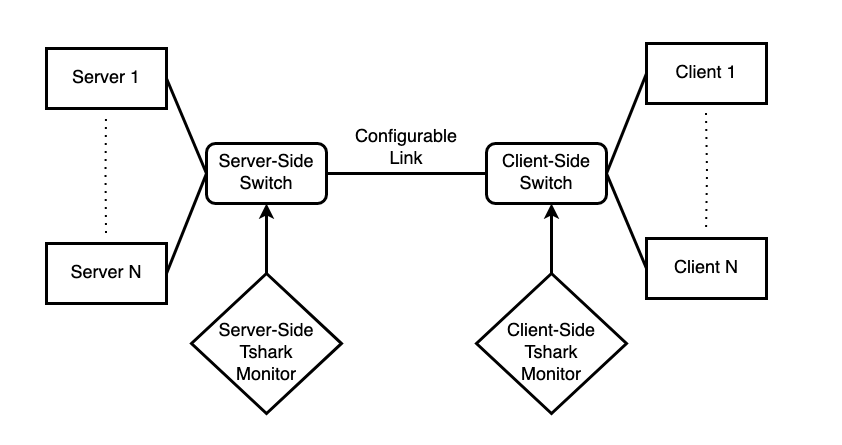
\includegraphics[scale=0.30]{Network_Topology.png}
  \end{center}
  
  \caption{\label{fig:Mininet}Mininet network topology used during testing. A configurable number of server nodes connect to a switch. A configurable number of client nodes connect to a separate switch. These switches are then connected via a central link. The properties (propagation delay, bandwidth, packet loss etc.) of the central link can be varied to simulate different network conditions.}
\end{figure}

\begin{figure*}
  \centering
  \begin{subfigure}[b]{0.32\textwidth}
      \centering
      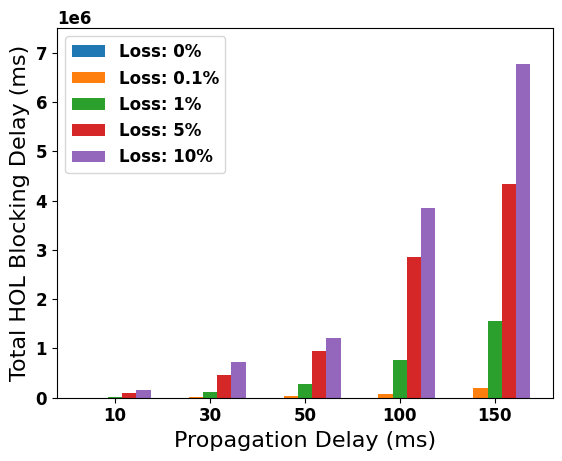
\includegraphics[width=\textwidth]{Total_HOL_Blocking/TCP_Total_HOL_delay.png}
      \caption{TCP: Total HOL blocking delay}
      \label{fig:TCP_HOL_TOTAL}
  \end{subfigure}
  \hfill
  \begin{subfigure}[b]{0.32\textwidth}
      \centering
      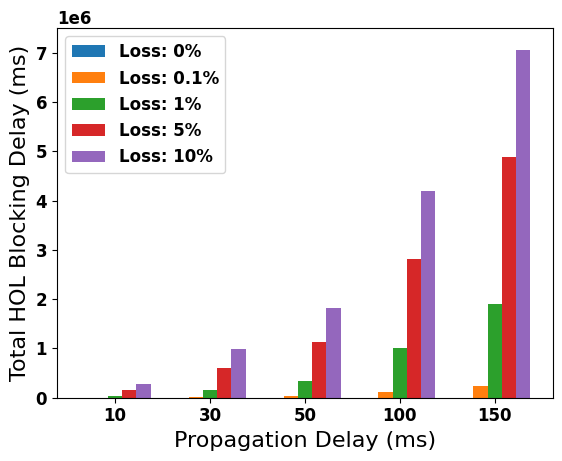
\includegraphics[width=\textwidth]{Total_HOL_Blocking/QUIC_SS_Total_HOL_delay.png}
      \caption{QUIC\_SS: Total HOL blocking delay}
      \label{fig:SS_HOL_TOTAL}
  \end{subfigure}
  \hfill
  \begin{subfigure}[b]{0.32\textwidth}
      \centering
      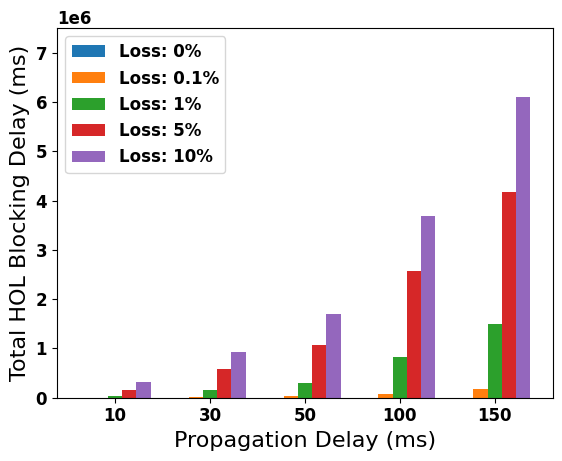
\includegraphics[width=\textwidth]{Total_HOL_Blocking/QUIC_GOP_Total_HOL_delay.png}
      \caption{QUIC\_GOP: Total HOL blocking delay}
      \label{fig:GOP_HOL_TOTAL}
  \end{subfigure}
  \begin{subfigure}[b]{0.32\textwidth}
      \centering
      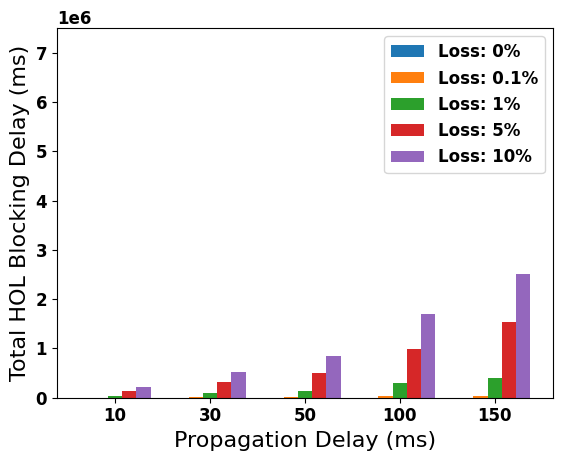
\includegraphics[width=\textwidth]{Total_HOL_Blocking/QUIC_FPS_Total_HOL_delay.png}
      \caption{QUIC\_FPS: Total HOL blocking delay}
      \label{fig:FPS_HOL_TOTAL}
  \end{subfigure}
  \hfill
  \begin{subfigure}[b]{0.32\textwidth}
      \centering
      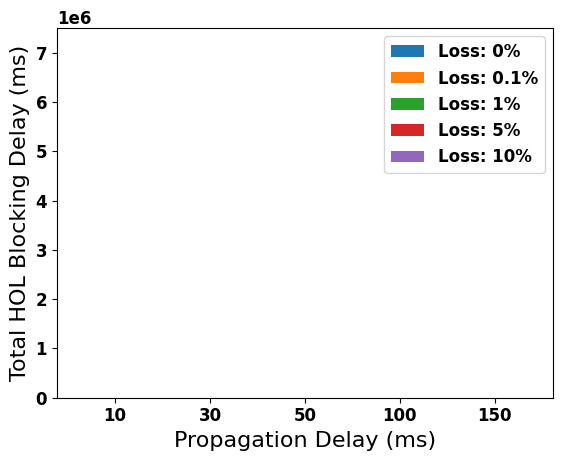
\includegraphics[width=\textwidth]{Total_HOL_Blocking/QUIC_PPS_Total_HOL_delay.png}
      \caption{QUIC\_PPS: Total HOL blocking delay}
      \label{fig:PPS_HOL_TOTAL}
  \end{subfigure}
  \hfill
  \begin{subfigure}[b]{0.32\textwidth}
      \centering
      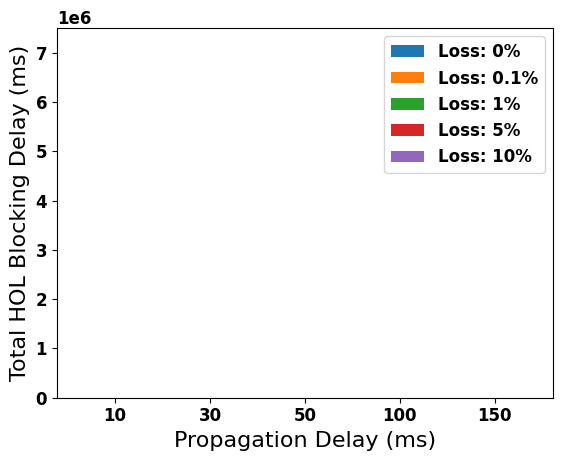
\includegraphics[width=\textwidth]{Total_HOL_Blocking/UDP_Total_HOL_delay.png}
      \caption{UDP: Total HOL blocking delay}
      \label{fig:UDP_HOL_TOTAL}
  \end{subfigure}
     \vspace{0.1cm}
     \centering
     \captionsetup{justification=centering, margin={1.5cm,0cm}}
     \caption{Bar plots showing the total HOL blocking delay for all packets for each implementation. Each group of bars represents a different packet propagation delay and the different colours denote the packet loss ratio on the link.}
     \label{fig:HOL_TOTAL}
\end{figure*}

\noindent To simulate the various network conditions, a custom dumbbell topology was created using Mininet's\footnote{http://mininet.org/} Python API (Figure \ref{fig:Mininet}). At the start of each test, the test framework would create a new Mininet instance, setting the parameters on the central link. TShark\footnote{https://www.wireshark.org/docs/man-pages/tshark.html} threads would then be started on both switch nodes to monitor network traffic. Both TShark instances would log their packet captures to the directory created for that test run. Unfortunately, it was common for the first few packets sent over the network to be missed by the TShark instances. To prevent the tests from losing any data, dummy network traffic was sent first using the iperf command.
\\\\
Once the network was initialised, the GStreamer pipelines would be started simultaneously on the server and client nodes. Each element in the pipelines would produce logs, which were stored for later analysis. The test framework would monitor the processes until the client-side pipeline completed its execution, indicating that the connection with the server had been terminated and any remaining video data had moved through the pipeline. If the pipeline failed to terminate within triple the run-time of the test video, it was assumed that a stall had occurred, and the process would be terminated manually.


\section{Results} \label{Results}


\subsection{The Impact of HOL Blocking} \label{The Impact of HOL Blocking}

\begin{figure*}
  \centering
  \begin{subfigure}[b]{0.32\textwidth}
      \centering
      \includegraphics[width=\textwidth]{SAL/TCP_Stack_Latency_Available.png}
      \caption{TCP: HOL blocking pattern}
      \label{fig:TSA}
  \end{subfigure}
  \hfill
  \begin{subfigure}[b]{0.32\textwidth}
      \centering
      \includegraphics[width=\textwidth]{SAL/QUIC_SS_Stack_Latency_Available.png}
      \caption{QUIC\_SS: HOL blocking pattern}
      \label{fig:SSSA}
  \end{subfigure}
  \hfill
  \begin{subfigure}[b]{0.32\textwidth}
      \centering
      \includegraphics[width=\textwidth]{SAL/QUIC_GOP_Stack_Latency_Available.png}
      \caption{QUIC\_GOP: HOL blocking pattern}
      \label{fig:GOPSA}
  \end{subfigure}
  \begin{subfigure}[b]{0.32\textwidth}
      \centering
      \includegraphics[width=\textwidth]{SAL/QUIC_FPS_Stack_Latency_Available.png}
      \caption{QUIC\_FPS: HOL blocking pattern}
      \label{fig:FPSSA}
  \end{subfigure}
  \hfill
  \begin{subfigure}[b]{0.32\textwidth}
      \centering
      \includegraphics[width=\textwidth]{SAL/QUIC_PPS_Stack_Latency_Available.png}
      \caption{QUIC\_PPS: HOL blocking pattern}
      \label{fig:PPSSA}
  \end{subfigure}
  \hfill
  \begin{subfigure}[b]{0.32\textwidth}
      \centering
      \includegraphics[width=\textwidth]{SAL/UDP_Stack_Latency_Available.png}
      \caption{UDP: HOL blocking pattern}
      \label{fig:USA}
  \end{subfigure}
     \vspace{0.1cm}
     \centering
     \captionsetup{justification=centering, margin={1.5cm,0cm}}
     \caption{Plots of packets against HOL blocking delay for the 14000-14500 packet range. Green lines indicate the start of a frame, Blue lines indicate the start of a GOP. Red dots indicate a loss event.}
     \label{fig:SA}
\end{figure*}

\noindent As the main benefit of the QUIC implementations presented in this paper is varying degrees of HOL blocking avoidance; it is important to use a metric that captures the impact of HOL blocking. This paper defines HOL blocking delay as the delay between a packet being sent by the server and that packet being made available to the application by the protocol stack on the client-side. To calculate this, a script was created that analysed server-side, and client-side packet captures. This method has an advantage over monitoring the application logs as the application may not read data as soon as it is available. By analysing the packet captures, the exact delay induced by HOL blocking for each packet can be calculated.
\\\\
Prior to the evaluation, the expectation was that TCP and \newline QUIC\_SS would be impacted the most by HOL blocking, as there should be no restriction on which subsequent packets are affected. QUIC\_GOP was expected to experience a lesser impact, as HOL blocking would not impact packets in other GOPs. However, the benefit would be minimal due to the size of GOPs. QUIC\_FPS was expected to significantly reduce HOL blocking delay, as loss would only impact individual frames. For each of these four implementations, the expectation was that HOL blocking delay would increase with both loss and propagation delay; A greater number of loss events results in more packet retransmissions and, as per equations (2) and (3), a higher propagation delay increases the retransmission time. Finally, it was expected that UDP and QUIC\_PPS would experience no HOL blocking at all, as UDP does not provide ordered delivery, and QUIC\_PPS sends an entire stream in each packet.
\\\\
The results conform to these expectations; Figure \ref{fig:HOL_TOTAL} above show the total HOL blocking delay experienced by each implementation across the entirety of the connection. Each group of bars represents a different packet propagation delay, and the different colours denote the packet loss ratio on the link. As the client-side buffer delay has no impact on the HOL blocking, these values were averaged across the five iterations for each client-side buffer delay value tested. As predicted, TCP (\ref{fig:TCP_HOL_TOTAL}) and QUIC\_SS (\ref{fig:SS_HOL_TOTAL}) were the most impacted, with the impact increasing with loss and propagation delay. QUIC\_GOP (\ref{fig:GOP_HOL_TOTAL}) sees a slight improvement, and QUIC\_FPS (\ref{fig:FPS_HOL_TOTAL}) shows a significant reduction in HOL blocking delay, reducing the total HOL blocking delay to under half of TCP and QUIC\_SS. Additionally, as expected, UDP (\ref{fig:UDP_HOL_TOTAL}) and QUIC\_PPS (\ref{fig:PPS_HOL_TOTAL}) experience no HOL blocking at all.

\subsubsection{Visualising HOL blocking} \label{Visualising HOL blocking}

\begin{figure*}
  \centering
  \begin{subfigure}[b]{0.32\textwidth}
      \centering
      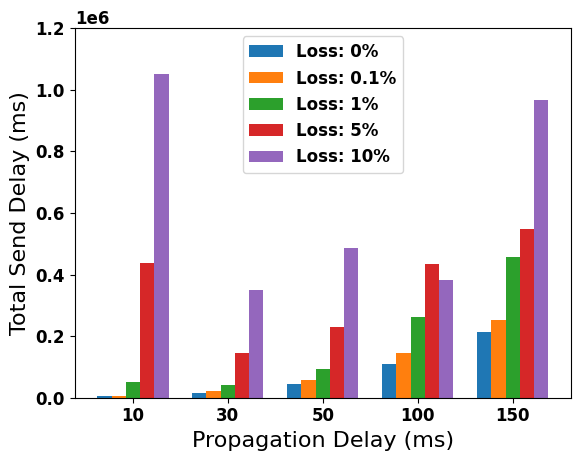
\includegraphics[width=\textwidth]{Total_Send/TCP/TCP_Total_Send_delay.png}
      \caption{TCP: Total sending delay}
      \label{fig:TCP_SEND}
  \end{subfigure}
  \hfill
  \begin{subfigure}[b]{0.32\textwidth}
      \centering
      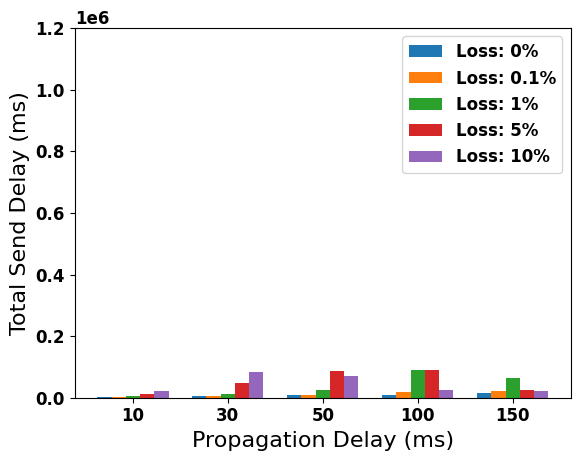
\includegraphics[width=\textwidth]{Total_Send/QUIC_SS/QUIC_SS_Total_Send_delay.png}
      \caption{QUIC\_SS: Total sending delay}
      \label{fig:SS_SEND}
  \end{subfigure}
  \hfill
  \begin{subfigure}[b]{0.32\textwidth}
      \centering
      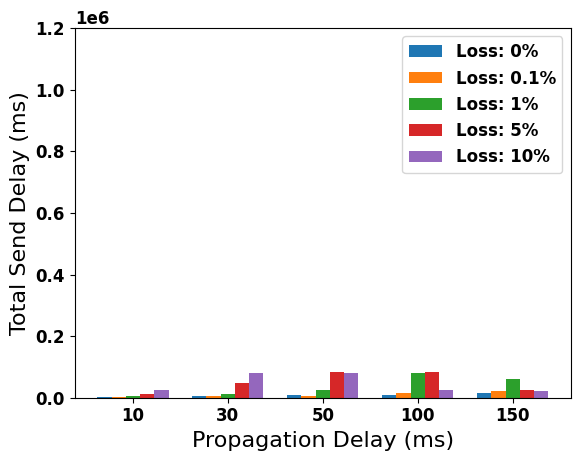
\includegraphics[width=\textwidth]{Total_Send/QUIC_GOP/QUIC_GOP_Total_Send_delay.png}
      \caption{QUIC\_GOP: Total sending delay}
      \label{fig:GOP_SEND}
  \end{subfigure}
  \begin{subfigure}[b]{0.32\textwidth}
      \centering
      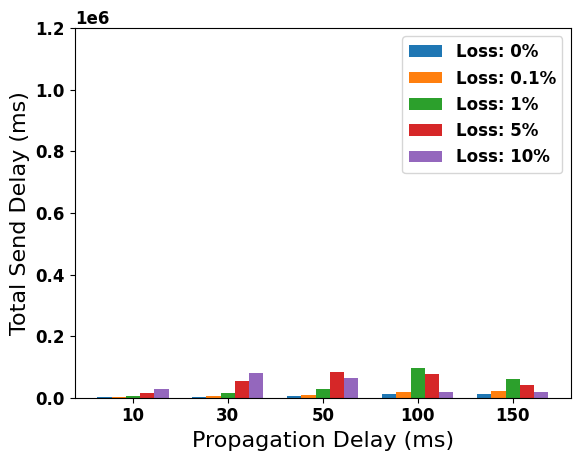
\includegraphics[width=\textwidth]{Total_Send/QUIC_FPS/QUIC_FPS_Total_Send_delay.png}
      \caption{QUIC\_FPS: Total sending delay}
      \label{fig:FPS_SEND}
  \end{subfigure}
  \hfill
  \begin{subfigure}[b]{0.32\textwidth}
      \centering
      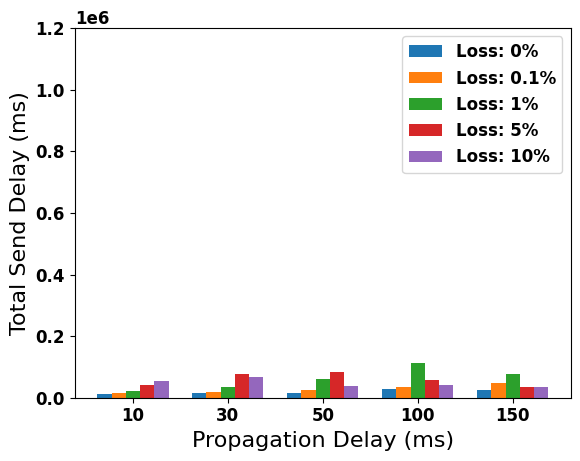
\includegraphics[width=\textwidth]{Total_Send/QUIC_PPS/QUIC_PPS_Total_Send_delay.png}
      \caption{QUIC\_PPS: Total sending delay}
      \label{fig:PPS_SEND}
  \end{subfigure}
  \hfill
  \begin{subfigure}[b]{0.32\textwidth}
      \centering
      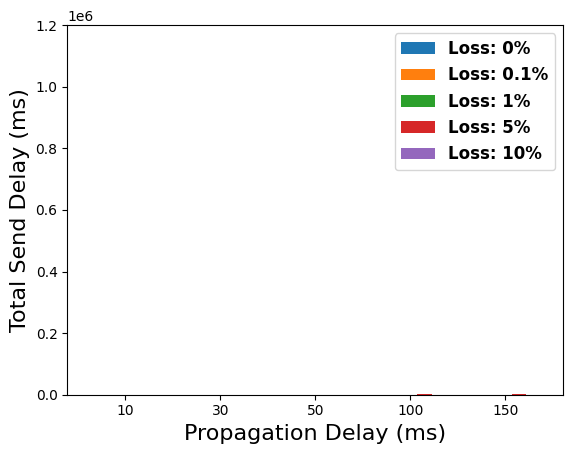
\includegraphics[width=\textwidth]{Total_Send/UDP/UDP_Total_Send_delay.png}
      \caption{UDP: Total sending delay}
      \label{fig:UDP_SEND}
  \end{subfigure}
     \vspace{0.1cm}
     \centering
     \captionsetup{justification=centering, margin={1.5cm,0cm}}
     \caption{Bar plots showing the total sending delay for all packets for each implementation. Each group of bars represents a different packet propagation delay and the different colours denote the packet loss ratio on the link.}
     \label{fig: SEND}
\end{figure*}


\noindent Figure \ref{fig:SA} provides visualisations of the HOL blocking delay patterns that are formed by different implementations. The plots are zoomed-in view on packets 14000 to 14500 as this makes it easier to view the patterns. The red dots indicate the HOL blocking delay for individual packets, the green lines indicate the start of frames, and the blue lines indicate the start of a new GOP. The test scenario with loss=1\% and propagation delay=100ms was chosen for display due to it providing the clearest representation of these patterns. However, the same patterns can be seen for any test scenarios that have loss greater than 0\%. 
\\\\
Figures \ref{fig:TSA} and \ref{fig:SSSA} demonstrate the impact of HOL blocking when only a single stream is used. After a loss occurs, a staircase pattern forms. Within frames, the HOL blocking delay will slowly decrease due to the small spacing between each packet. Between frames, we see a roughly 41.6667ms drop in the HOL blocking delay due to the spacing between each frame. As HOL blocking is not mitigated at all in these implementations, after a loss occurs, subsequent packets are delayed by the protocol stack until the lost packet arrives. As the figures show, the later a packet is sent when compared to the lost packet; the less HOL blocking will impact it. If a subsequent packet is also lost, then the pattern will restart. As mentioned above, this pattern can be seen for all loss values greater than 0\%. As propagation delay increases, so does the retransmission time, so the staircase pattern begins at a higher point. As loss increases, the frequency at which the staircase pattern restarts also increases.
\\\\
Moving on to figure \ref{fig:GOPSA}, the benefits of eliminating HOL blocking between GOPs can be seen. The graph is mostly similar to figures \ref{fig:TSA} and \ref{fig:SSSA}; however, there is one key difference. The staircase pattern will not continue when a new GOPs begins. This can significantly reduce the number of packets impacted by HOL blocking in certain cases, and this is best demonstrated by the behaviour of \ref{fig:GOPSA} around packet number 14100. However, the duration of a GOP is typically much longer than a single frame, and as a result, the majority of packets that are sent after a loss event are still impacted.
\\\\
Figure \ref{fig:FPSSA} shows the stack latency availability for QUIC\_FPS. HOL blocking is contained within frames, and the staircase pattern seen in the figures for TCP, QUIC\_SS and QUIC\_GOP has disappeared. This demonstrates the substantial reduction in HOL blocking delay achieved by\newline QUIC\_FPS, which aligns with the results shown in section \ref{The Impact of HOL Blocking}. QUIC\_PPS goes even further, completely eliminating HOL blocking delays, as can be seen in figure \ref{fig:PPSSA}. When using QUIC\_PPS, as is the case with UDP (figure \ref{fig:USA}), the only packet affected by loss, is the lost packet itself.
\\\\
It should be noted that, while lost packets do impact other packets within the same frame when using QUIC\_FPS, the majority of these packets will not be useful until the missing packet arrives. The exception is the case that the lost packet carries all or part of a redundant NAL unit, and this is where QUIC\_PPS provides an advantage.

% \begin{figure}[tbp]
%   \centering
%   \captionsetup{justification=centering, margin={1.3cm,0cm}}
%   \includegraphics[scale=0.55]{TCP_Stack_Latency_Available.png}
%   \caption{\label{fig:TSA}TCP HOL blocking delay\newline Loss: 1\%, Delay 100ms}

%   \includegraphics[scale=0.55]{QUIC_GOP_Stack_Latency_Available.png}
%   \caption{\label{fig:GOPSA}QUIC\_GOP HOL blocking delay\newline Loss: 1\%, Delay 100ms}

%   \includegraphics[scale=0.55]{QUIC_PPS_Stack_Latency_Available.png}
%   \caption{\label{fig:PPSSA}QUIC\_PPS HOL blocking delay\newline Loss: 1\%, Delay 100ms}
% \end{figure}

% \begin{figure}[tbp]
%   \centering
%   \captionsetup{justification=centering, margin={1.5cm,0cm}}
%   \includegraphics[scale=0.55]{QUIC_SS_Stack_Latency_Available.png}
%   \caption{\label{fig:SSSA}QUIC\_SS HOL blocking delay\newline Loss: 1\%, Delay 100ms}

%   \includegraphics[scale=0.55]{QUIC_FPS_Stack_Latency_Available.png}
%   \caption{\label{fig:FPSSA}QUIC\_FPS HOL blocking delay\newline Loss: 1\%, Delay 100ms}

%   \includegraphics[scale=0.55]{UDP_Stack_Latency_Available.png}
%   \caption{\label{fig:USA}UDP HOL blocking delay\newline Loss: 1\%, Delay 100ms}
% \end{figure}


\subsection{Sending Delay}

\begin{figure*}
  \centering
  \begin{subfigure}[b]{0.25\textwidth}
      \centering
      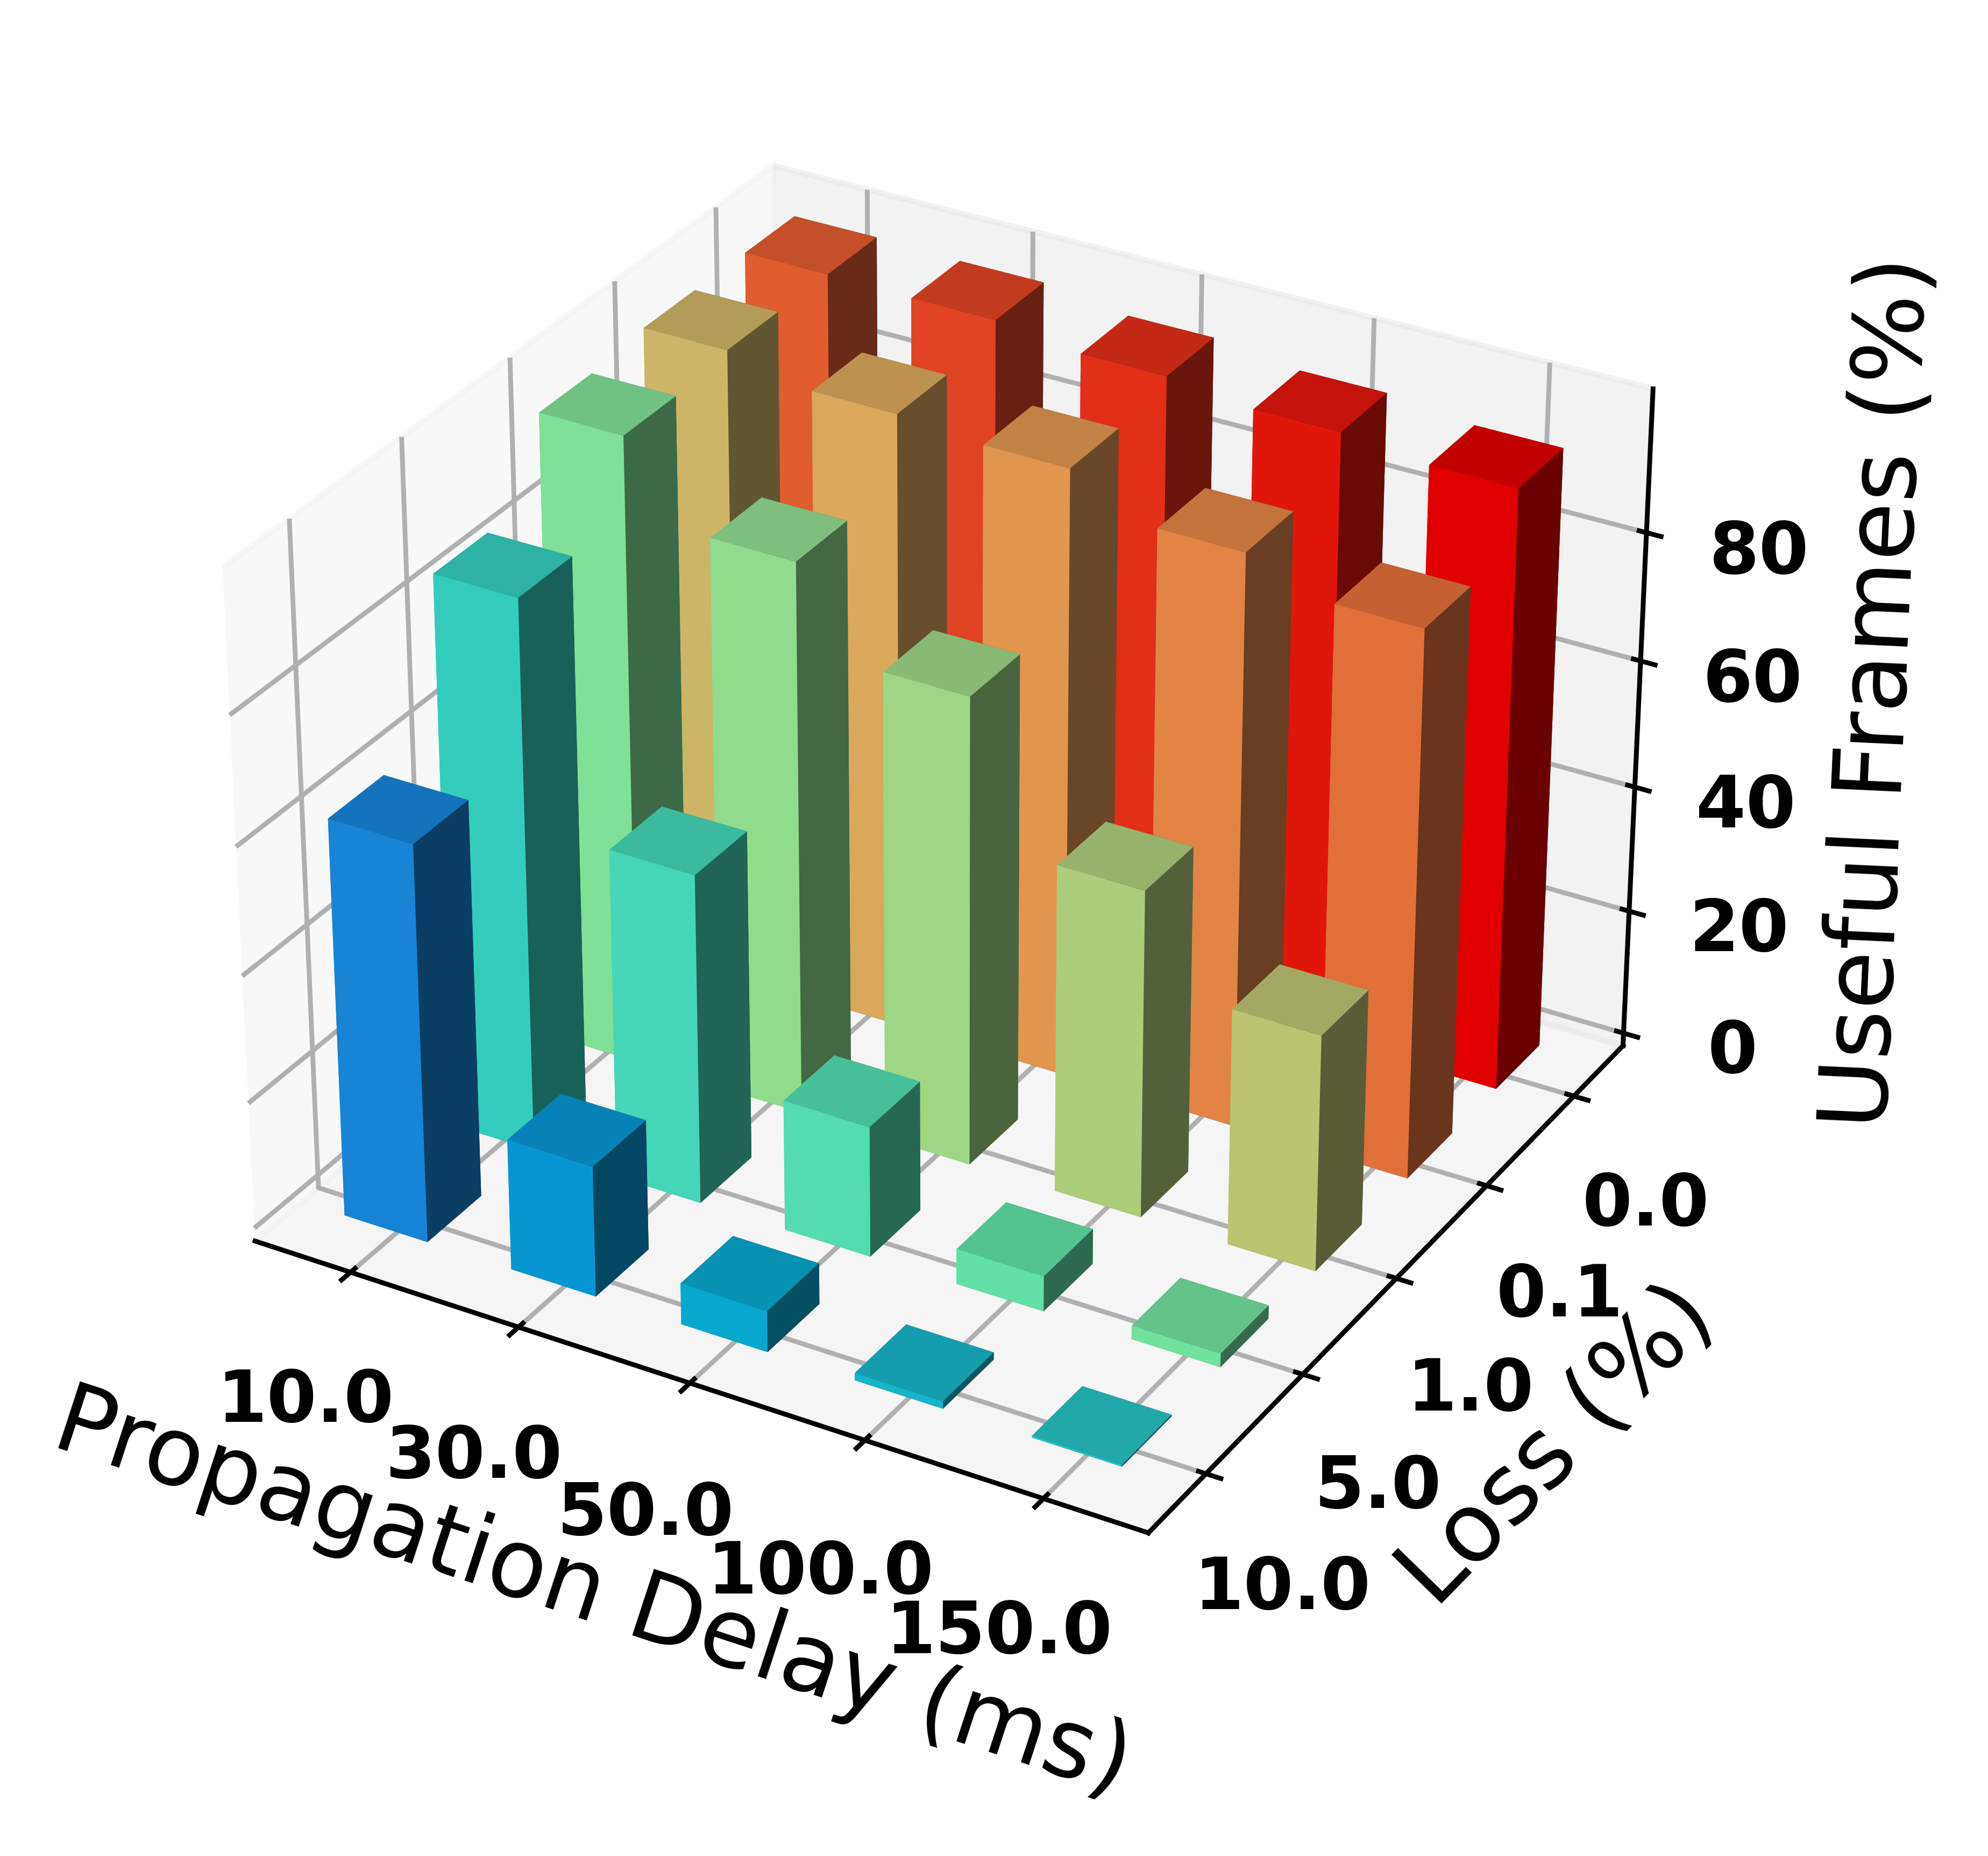
\includegraphics[width=\textwidth]{Frame_Usefulness_Ratio/TCP/AVG_Frame_Usefulness-42.png}
      \caption{TCP: Useful Frames}
      \label{fig:TCP_bar-42}
  \end{subfigure}
  \hfill
  \begin{subfigure}[b]{0.25\textwidth}
      \centering
      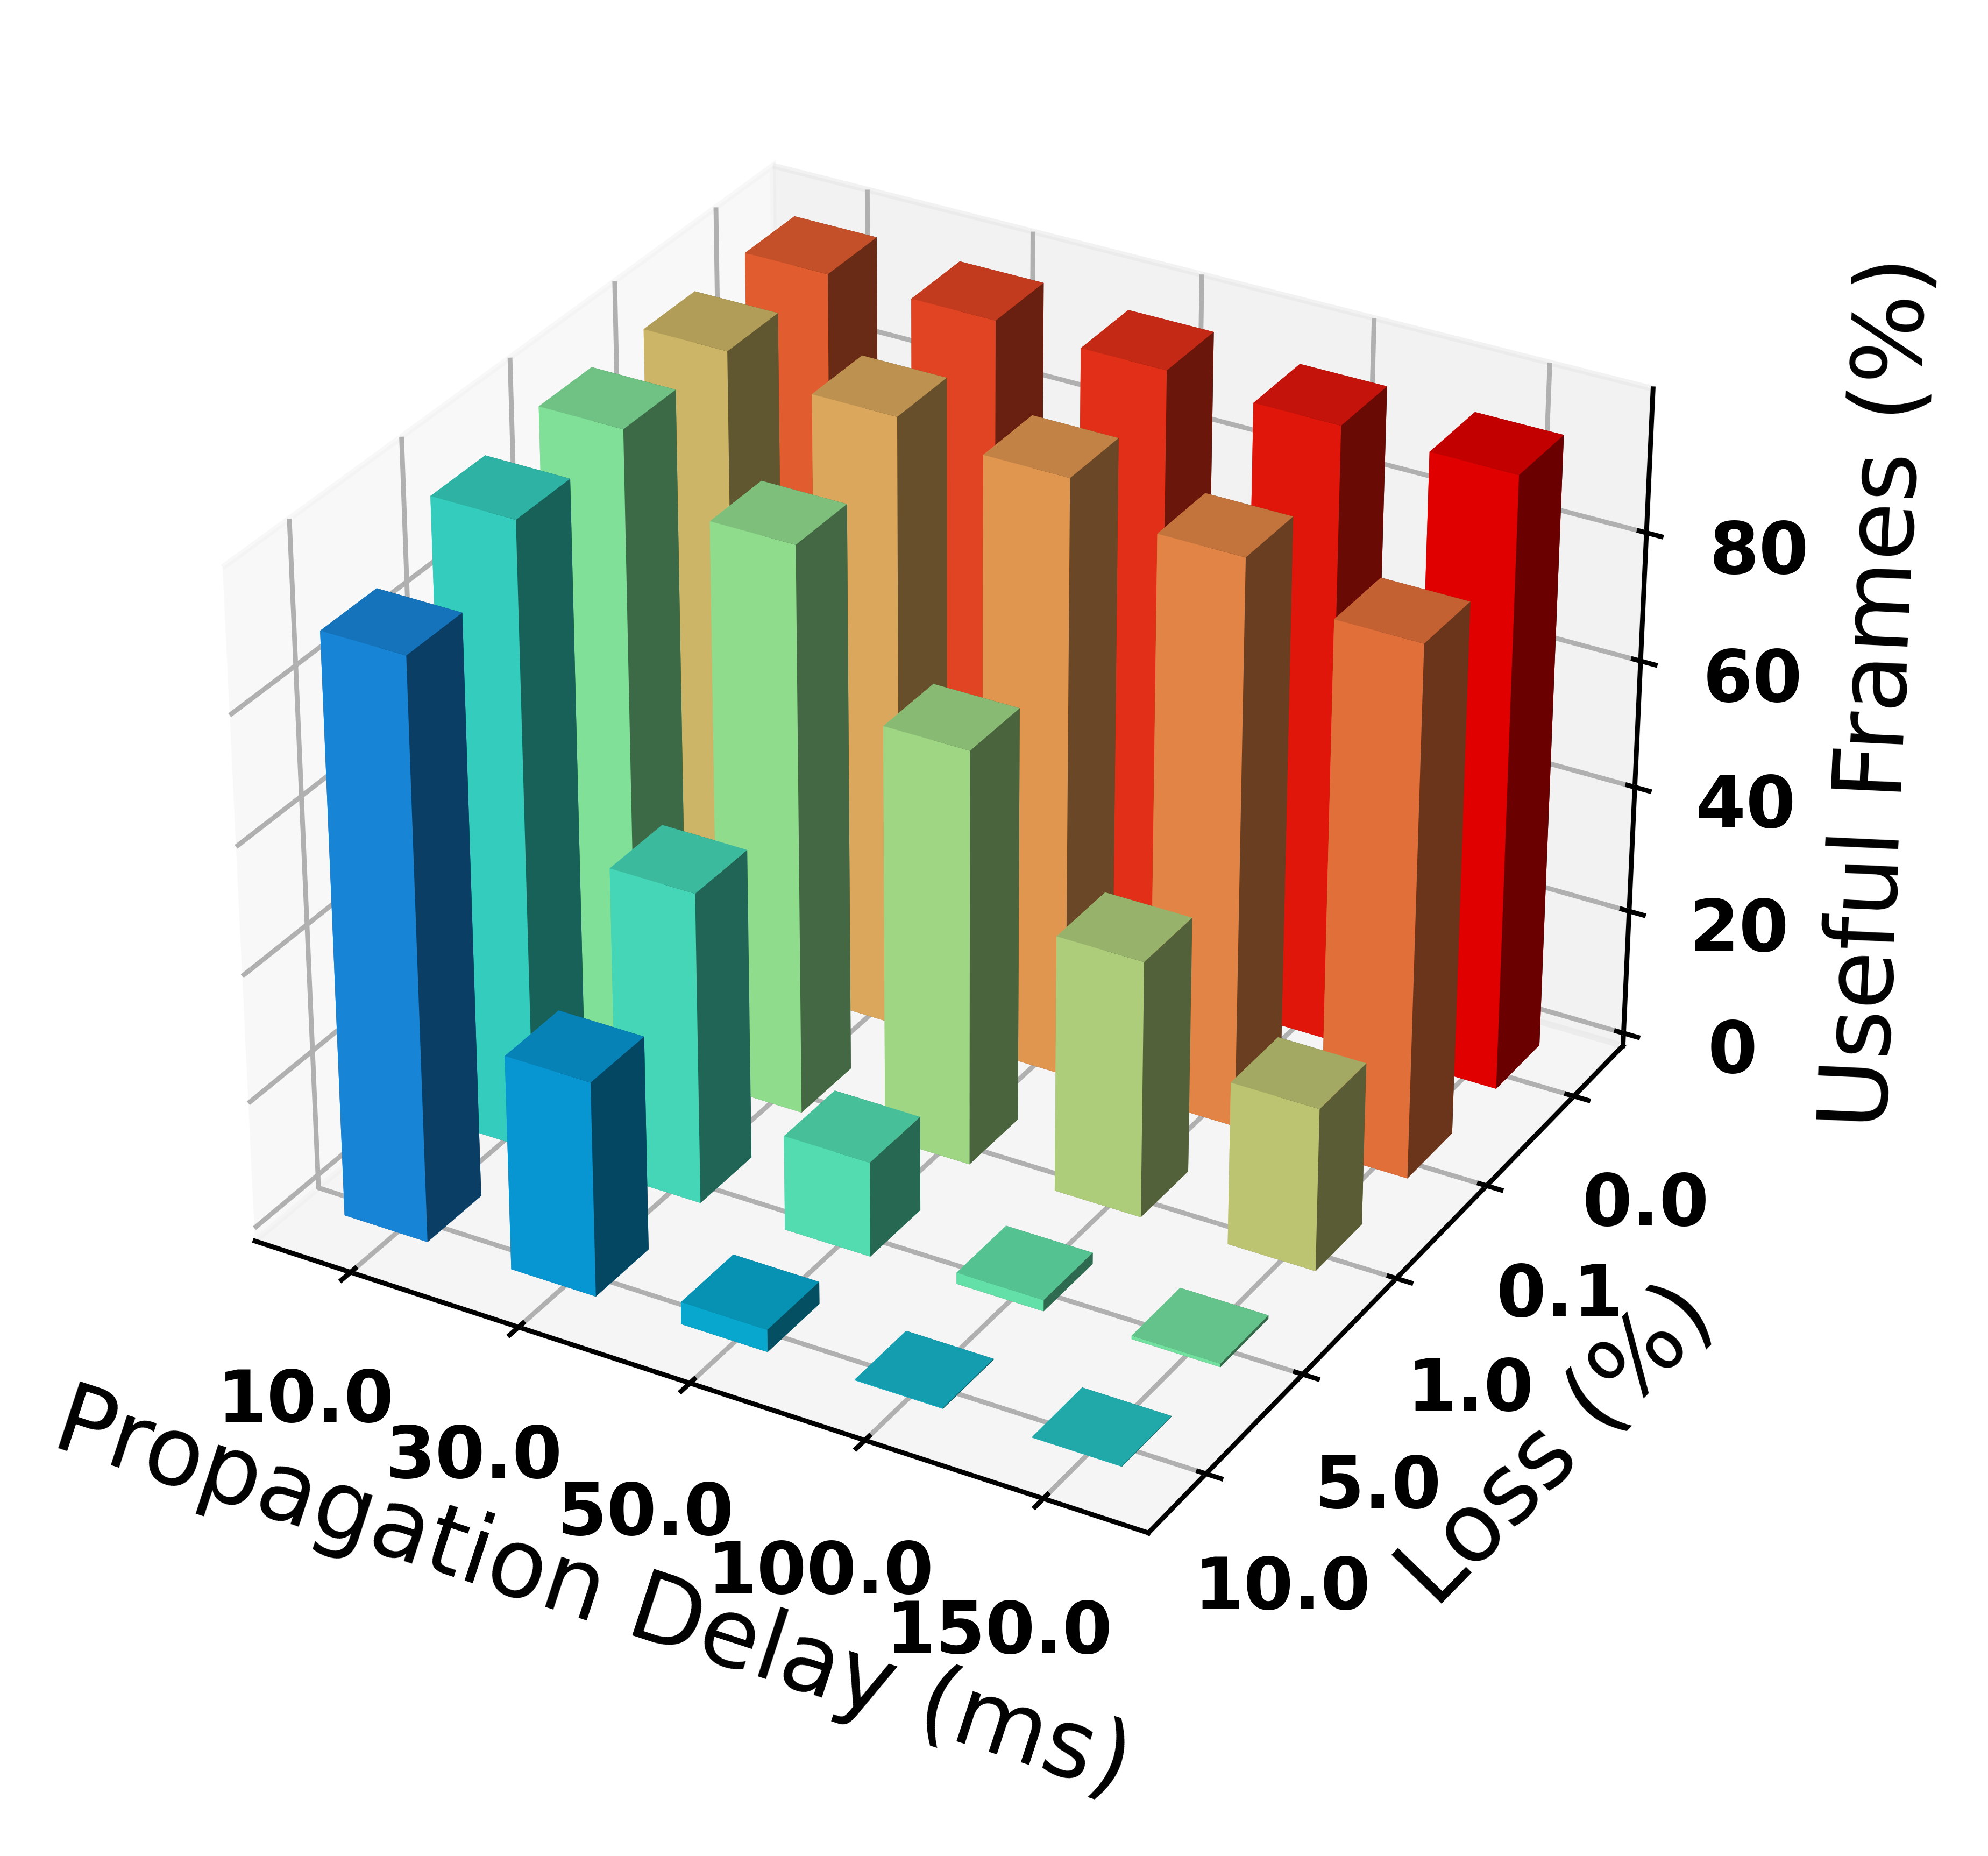
\includegraphics[width=\textwidth]{Frame_Usefulness_Ratio/QUIC_SS/AVG_Frame_Usefulness-42.png}
      \caption{QUIC\_SS: Useful Frames}
      \label{fig:SS_bar-42}
  \end{subfigure}
  \hfill
  \begin{subfigure}[b]{0.25\textwidth}
      \centering
      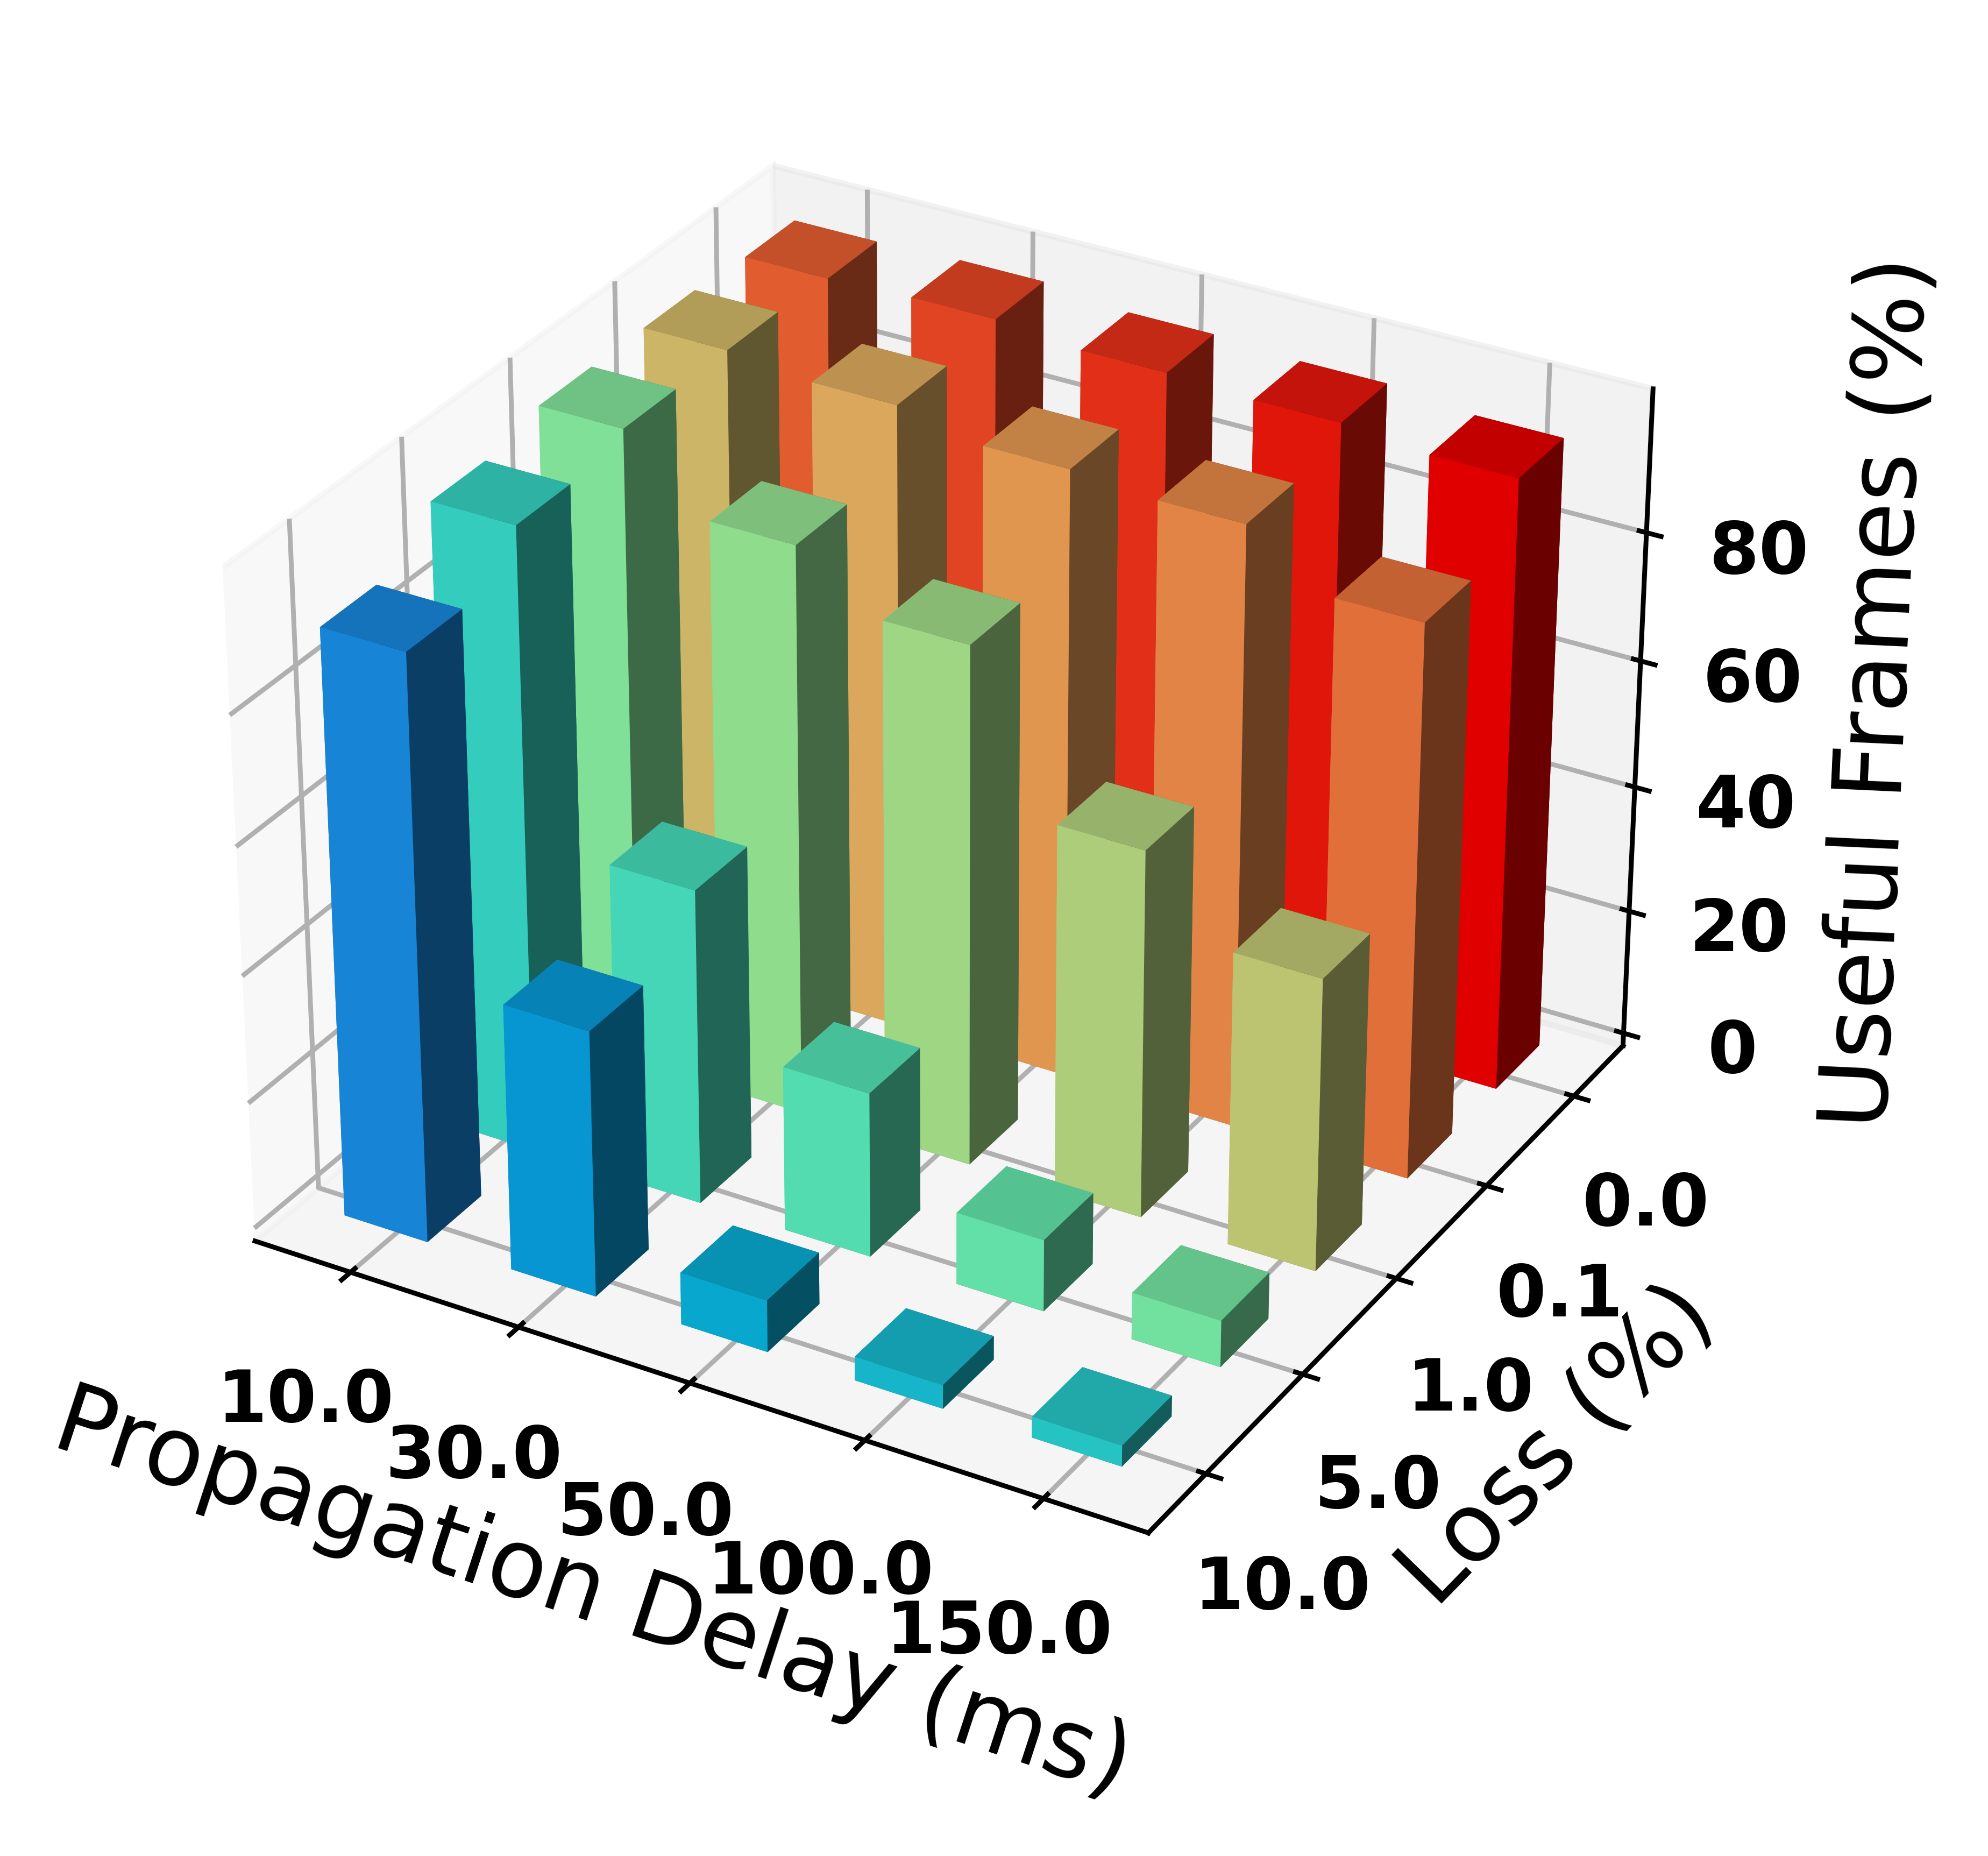
\includegraphics[width=\textwidth]{Frame_Usefulness_Ratio/QUIC_GOP/AVG_Frame_Usefulness-42.png}
      \caption{QUIC\_GOP: Useful Frames}
      \label{fig:GOP_bar-42}
  \end{subfigure}
  \begin{subfigure}[b]{0.25\textwidth}
      \centering
      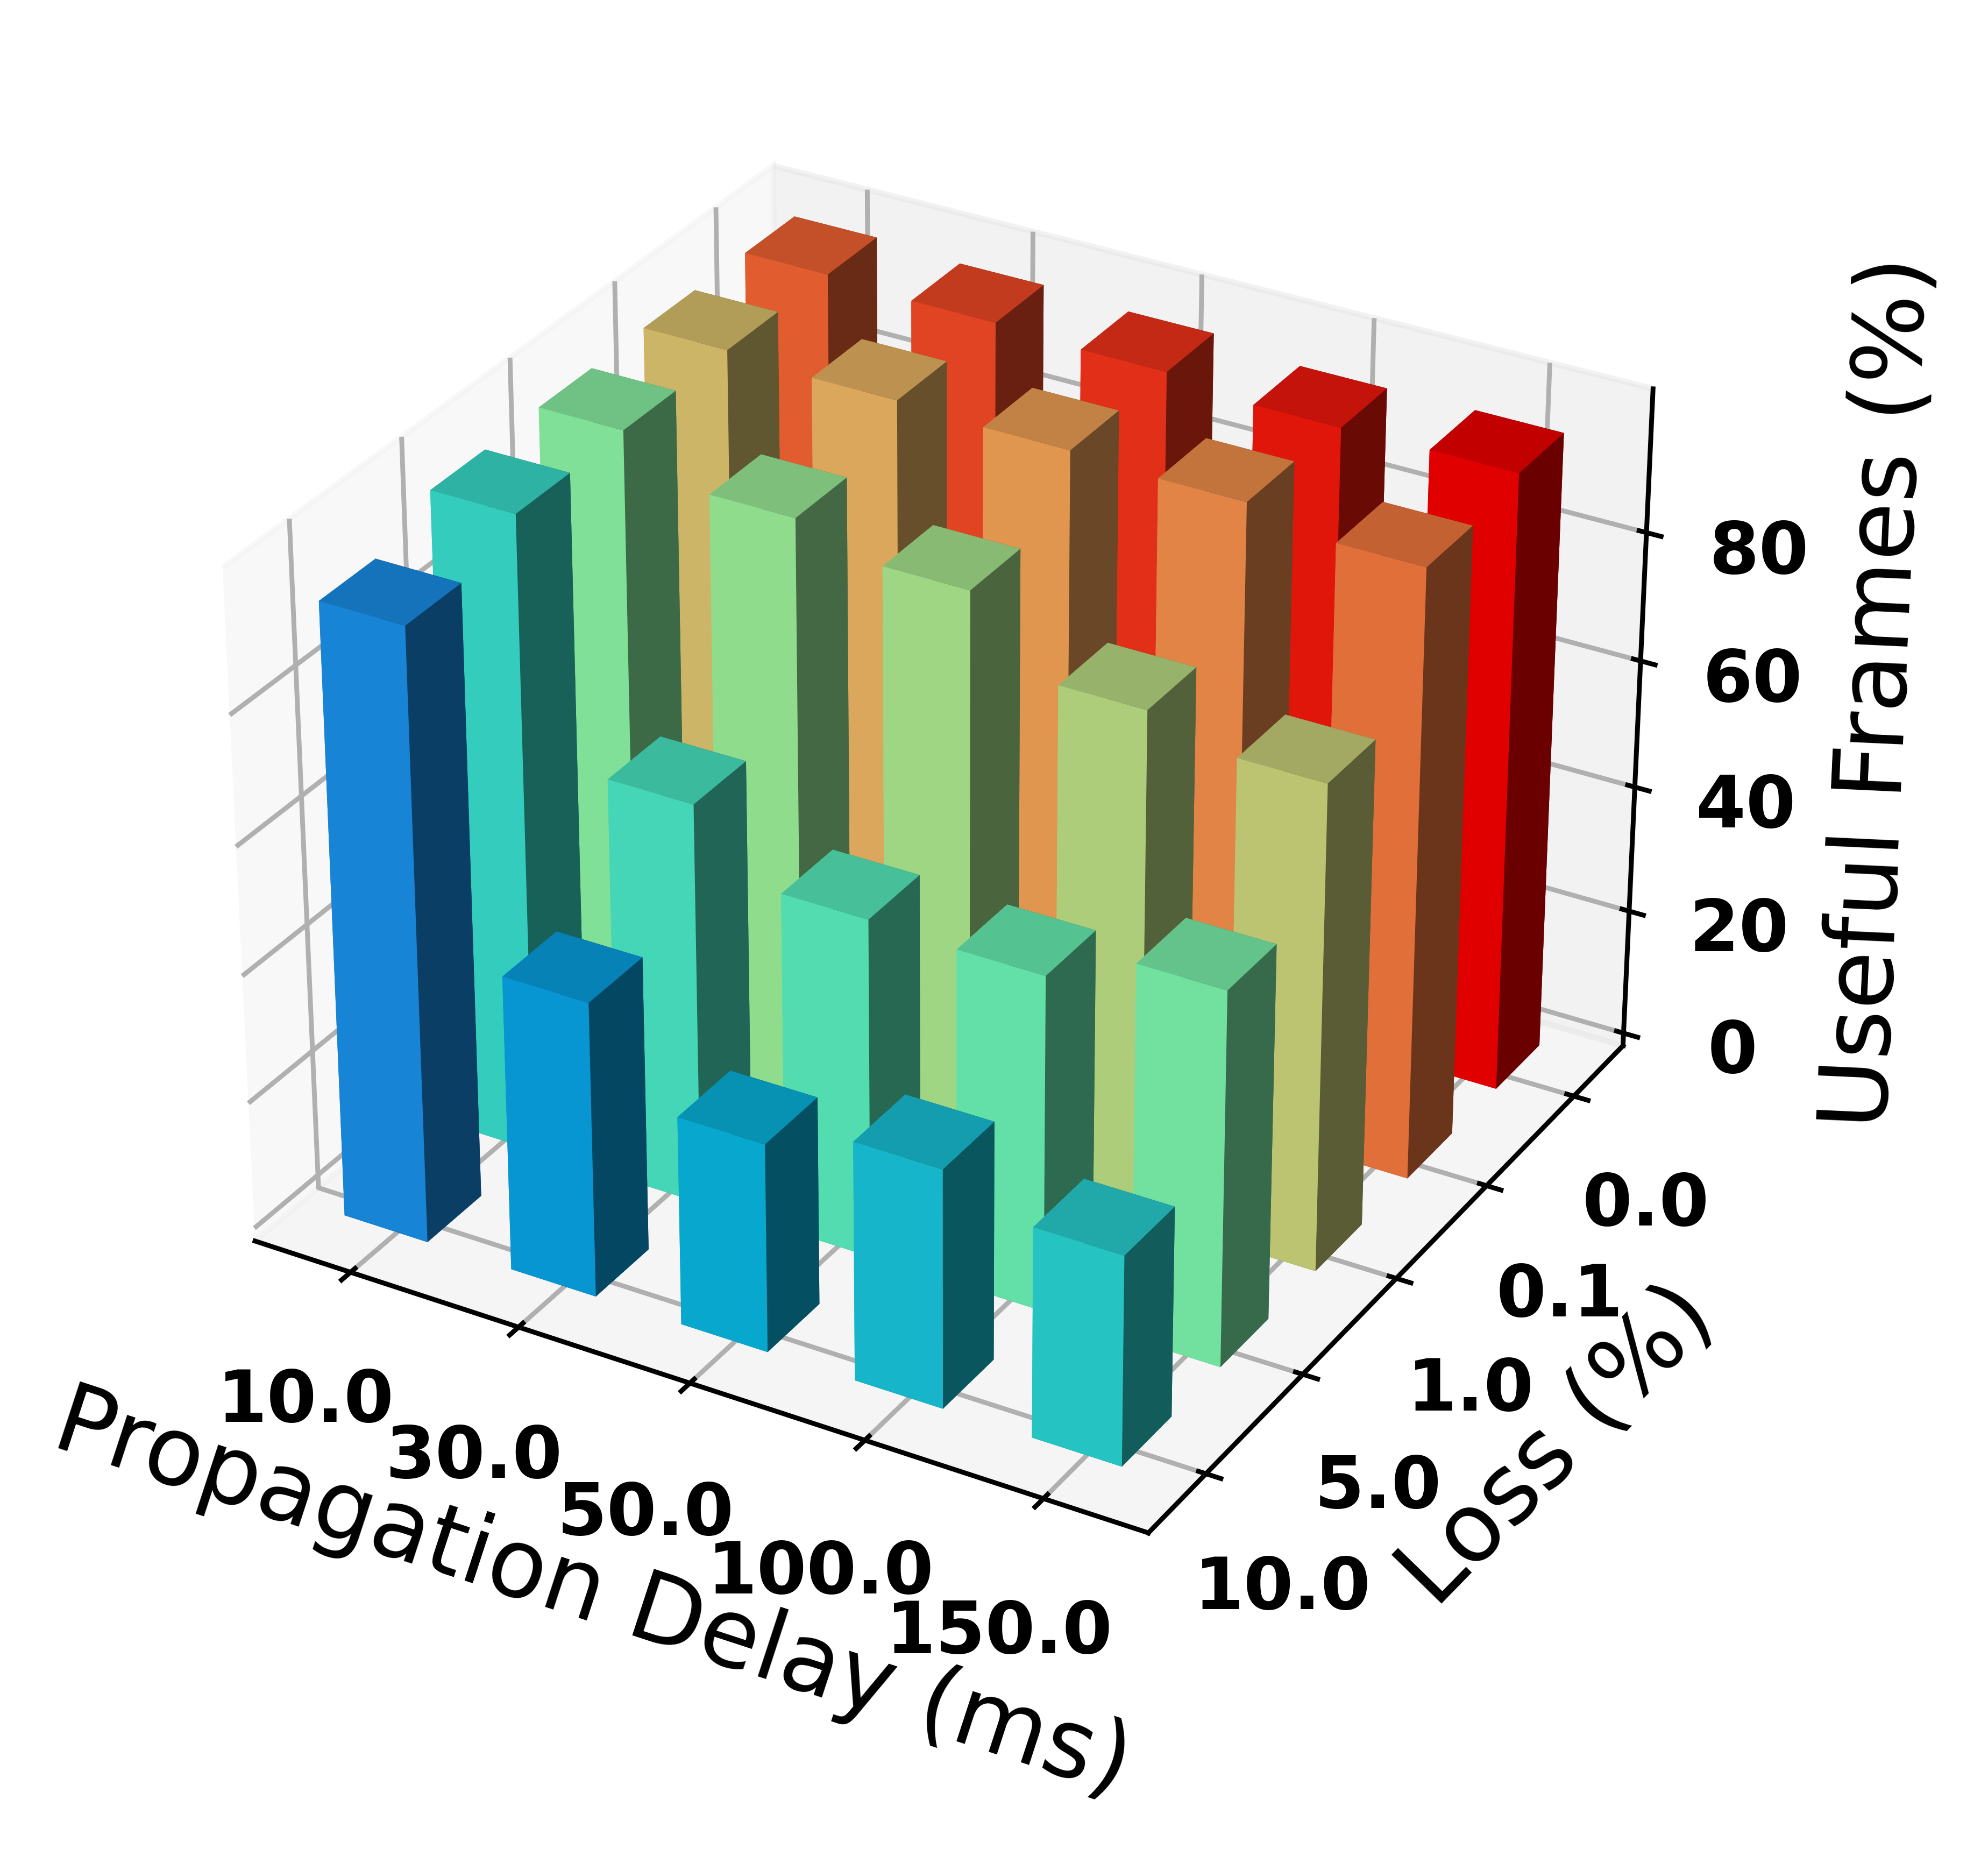
\includegraphics[width=\textwidth]{Frame_Usefulness_Ratio/QUIC_FPS/AVG_Frame_Usefulness-42.png}
      \caption{QUIC\_FPS: Useful Frames}
      \label{fig:FPS_bar-42}
  \end{subfigure}
  \hfill
  \begin{subfigure}[b]{0.25\textwidth}
      \centering
      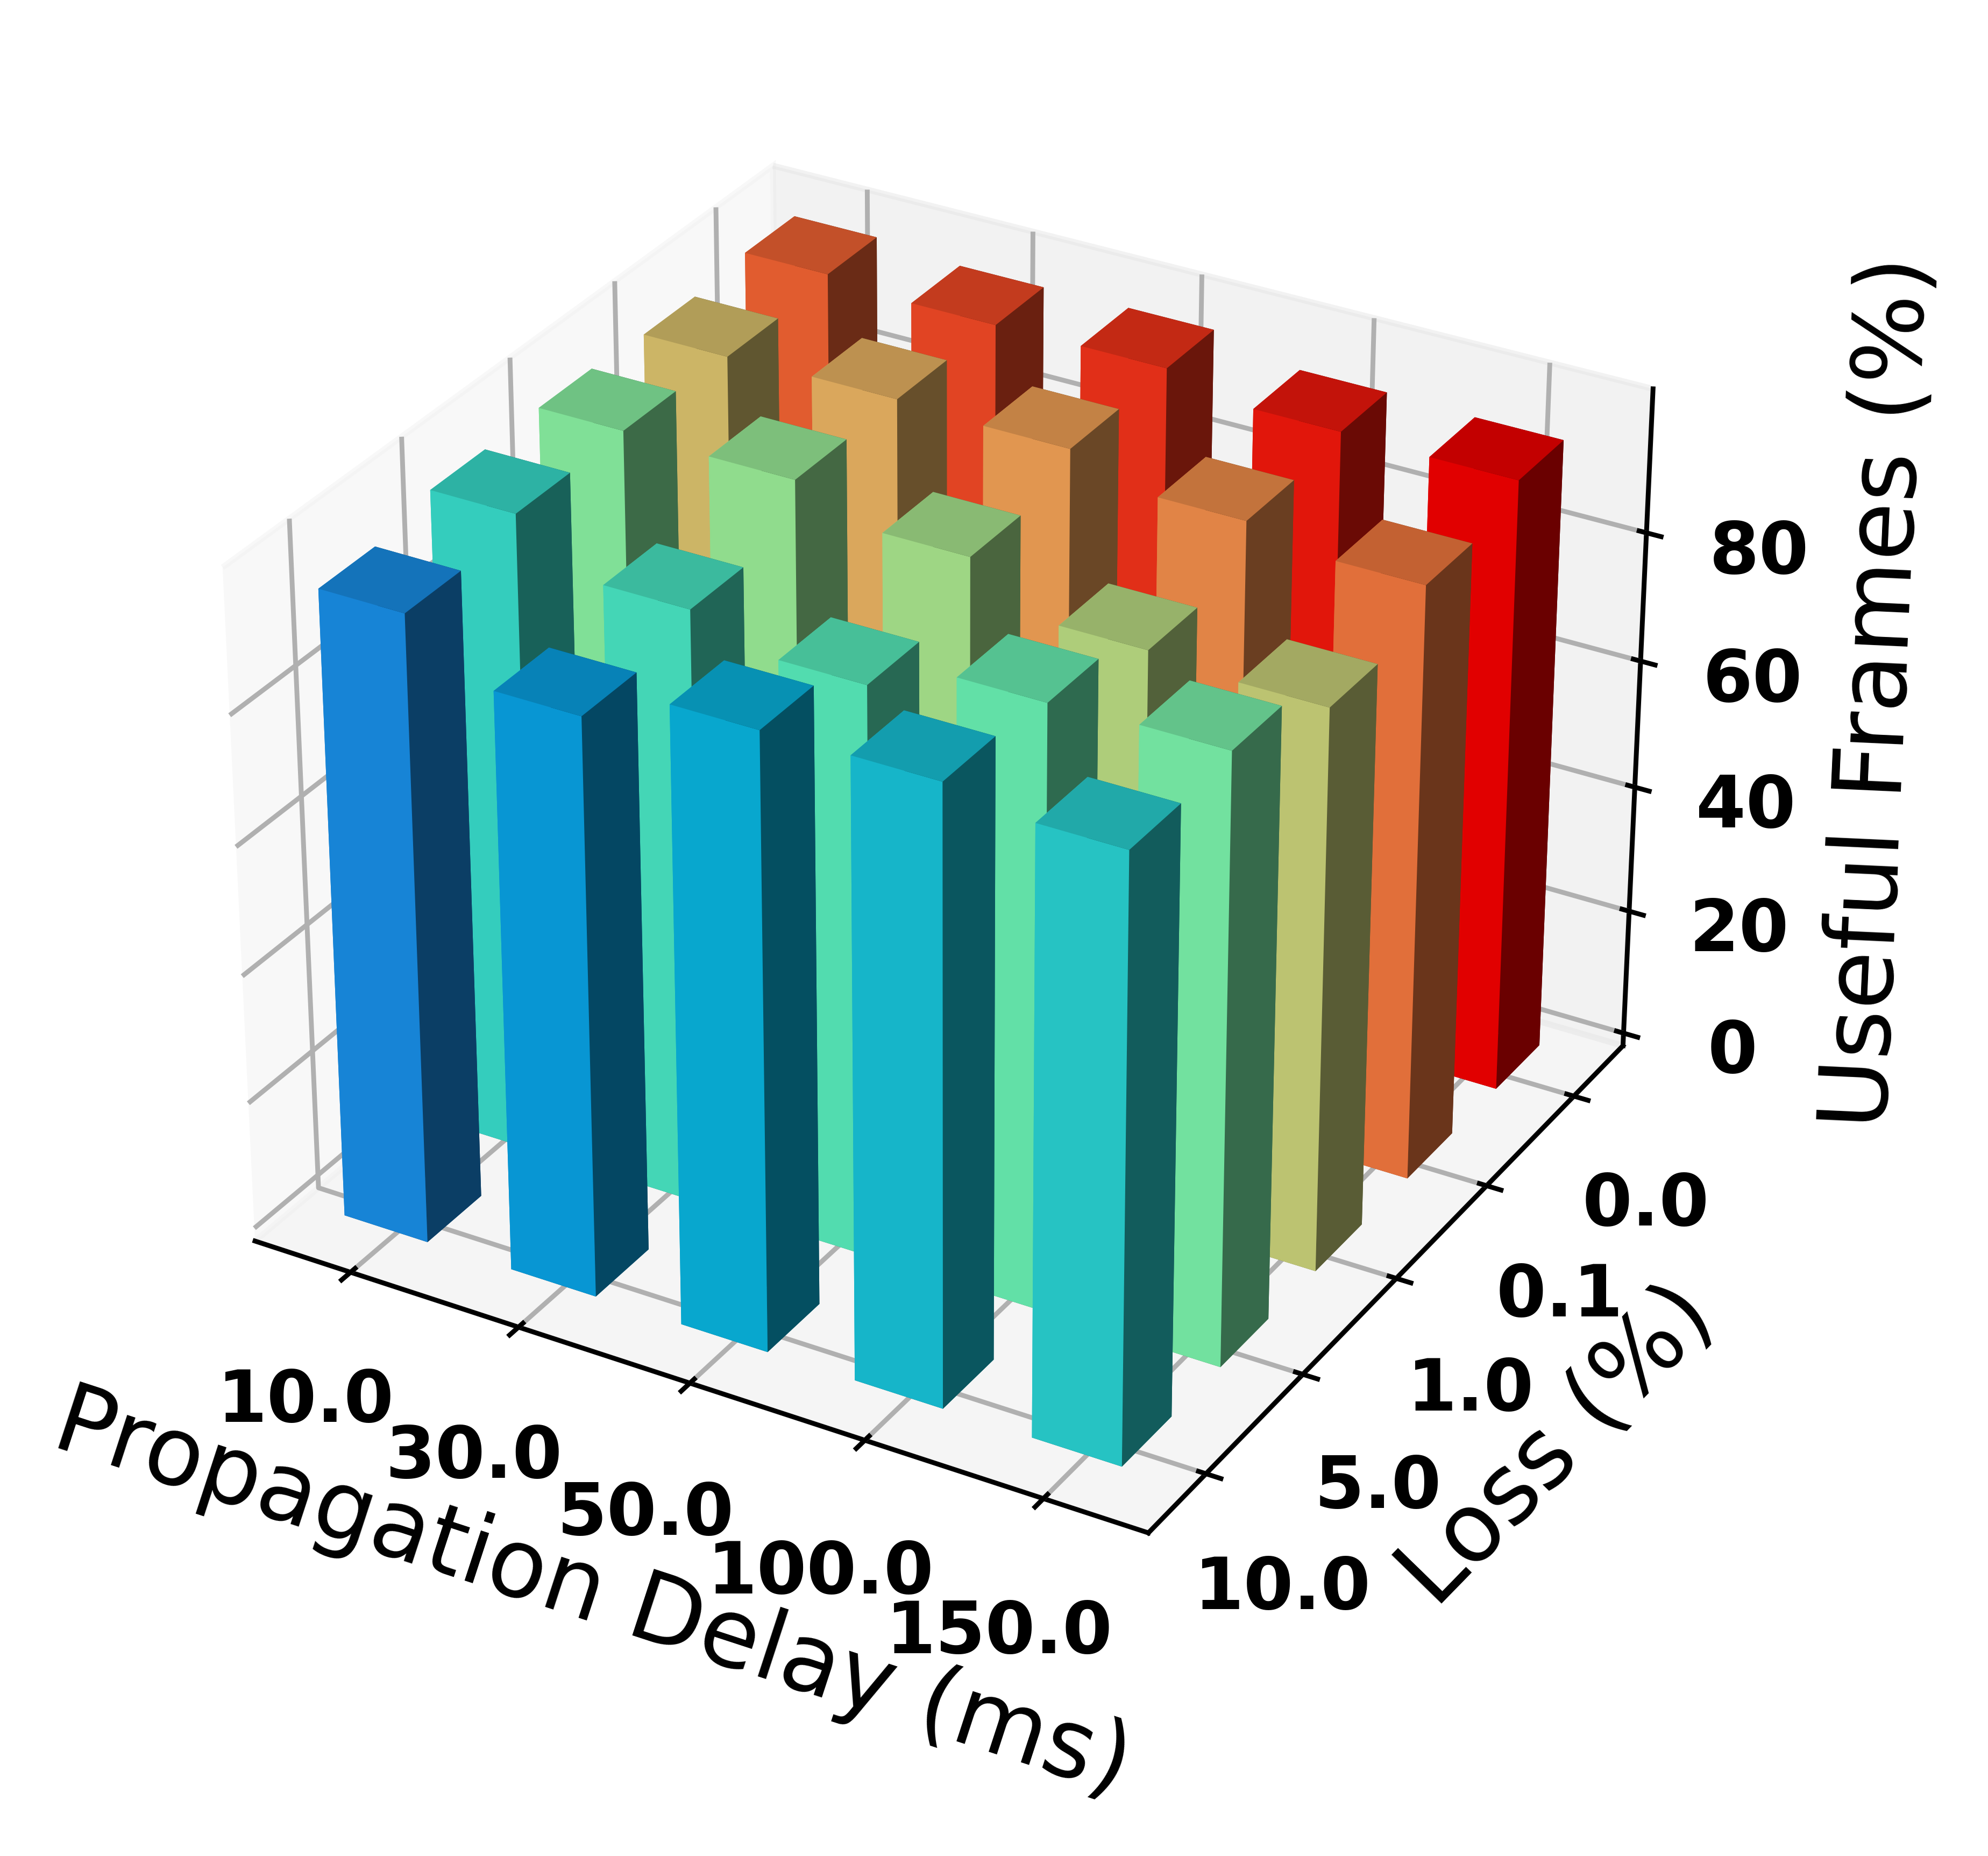
\includegraphics[width=\textwidth]{Frame_Usefulness_Ratio/QUIC_PPS/AVG_Frame_Usefulness-42.png}
      \caption{QUIC\_PPS: Useful Frames}
      \label{fig:PPS_bar-42}
  \end{subfigure}
  \hfill
  \begin{subfigure}[b]{0.25\textwidth}
      \centering
      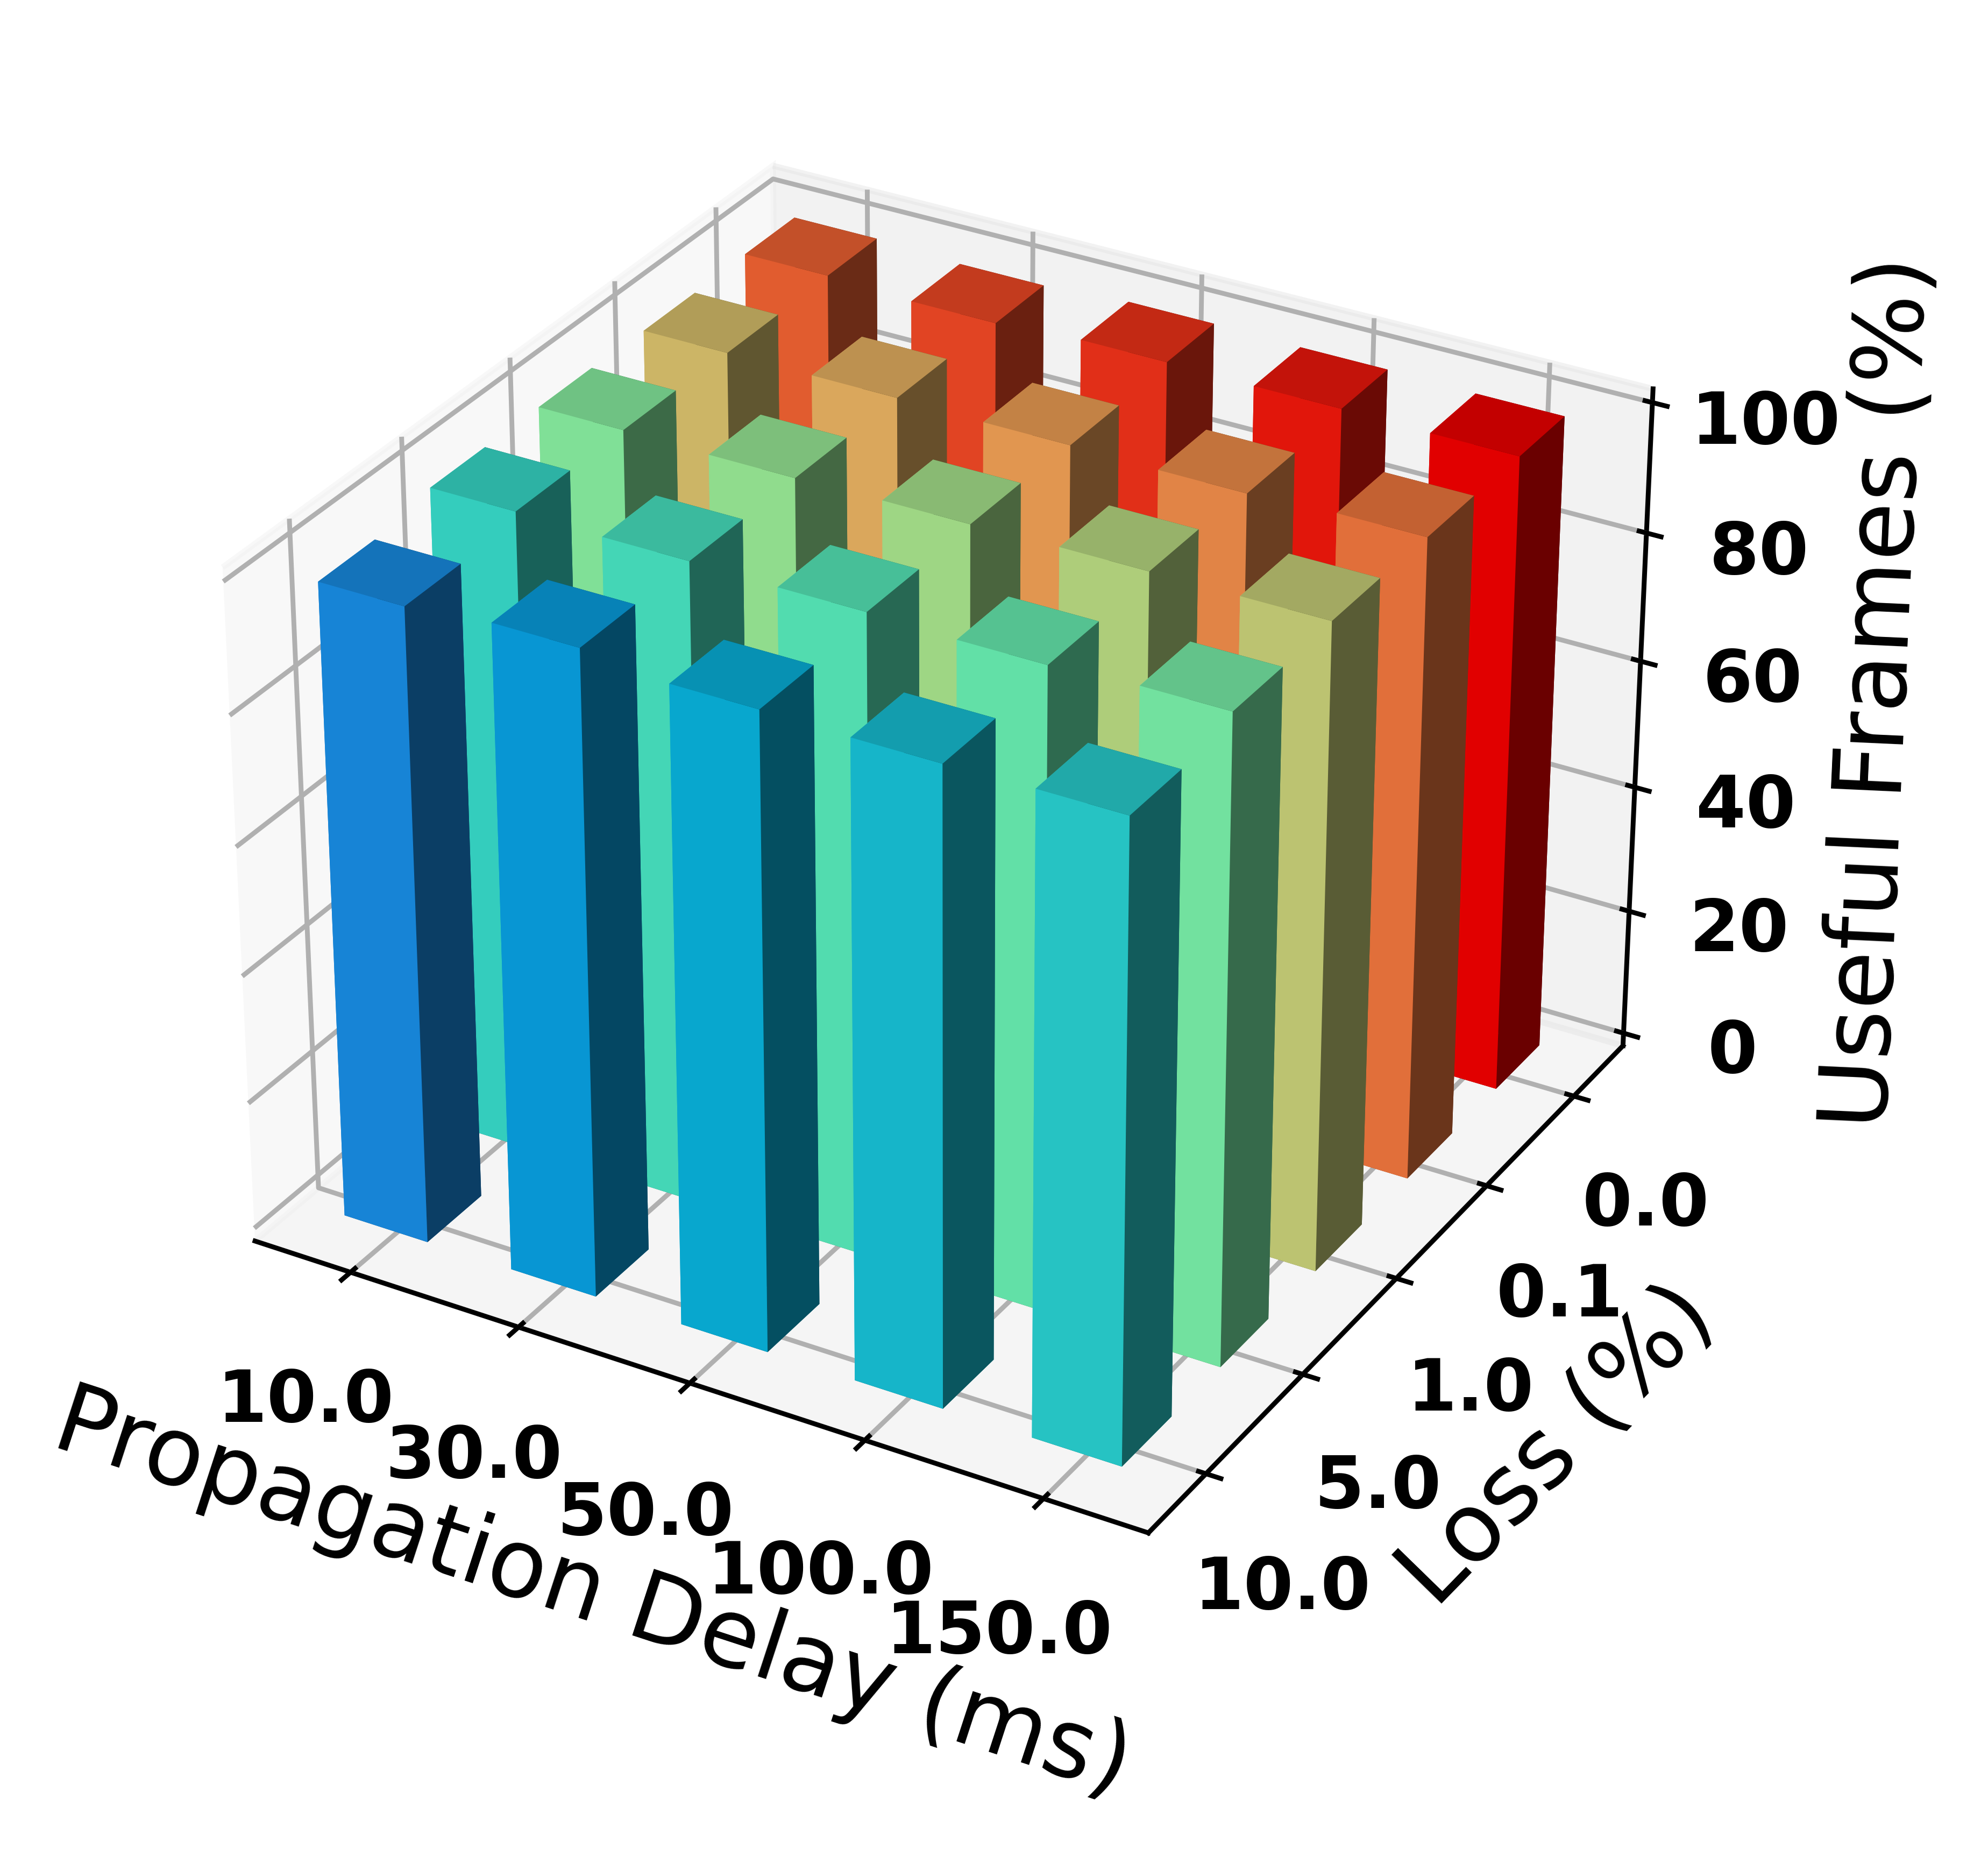
\includegraphics[width=\textwidth]{Frame_Usefulness_Ratio/UDP/AVG_Frame_Usefulness-42.png}
      \caption{UDP: Useful Frames}
      \label{fig:UDP_bar-42}
  \end{subfigure}
     \vspace{0.1cm}
     \centering
     \captionsetup{justification=centering, margin={1.5cm,0cm}}
     \caption{3d bar plots showing the percentage of useful frames delivered by each implementation at different levels of loss and propagation delay. The receive buffer size for these tests was 42ms.}
     \label{fig: 42-bar}
\end{figure*}

\noindent In the previous subsection, the paper examined the impact of HOL blocking, which injects delay at the client-side. In this subsection, the paper explores the impact of the BBR congestion control algorithm on the sending rate of video data. Flow control could also introduce delays at the server-side. However, as discussed within section \ref{Implementation}, the flow control values were configured such that flow control would not impact the sending rate. This allows the effect of congestion control on the sending delay to be isolated.
\\\\
To calculate the sending delay of each packet, the time difference between an RTP packet being passed to the network protocol stack and the packet being sent was determined for each packet. The expectation was that QUIC and TCP would show some sending delay due to BBR even when loss was zero, due to the periodic PROBERTT state. As the propagation delay increases, the impact of the PROBERTT state will also increase (As more time will be required for all packets in flight to be acknowledged). Additionally, it was expected that higher loss values would lead to a greater sending delay, as BBR would enter loss recovery and reduce its sending rate. Finally, no significant difference was expected between each QUIC implementation and TCP, as they all utilise the same congestion control algorithm.
\\\\
Surprisingly, while the expectation that QUIC and TCP would experience some sending delay on lossless networks held true, the results showed some significant deviation from the other expectations. Similar to Figure \ref{fig:HOL_TOTAL}, Figure \ref{fig: SEND} shows the total sending delay experienced by each implementation across the entirety of the connection. Each group of bars represents a different propagation delay, and the different colours denote the packet loss ratio on the link. As the client-side buffer delay has no impact on the HOL blocking, these values were averaged across the five iterations for each client-side buffer delay value tested. Looking at figure \ref{fig: SEND}, three major deviations from our expectations can be observed: 1) TCP is impacted by its congestion control significantly more than the QUIC implementations; 2) On small delay but high loss links (propagation delay = 10ms), TCP sees a much higher total sending delay than seen on higher latency links; 3) At higher latencies, the QUIC implementations are impacted less by the congestion control when loss is at 1\% than at higher loss values.
\\\\
The reason for deviation 3 is related to how BBR handles loss recovery. As mentioned in \ref{Congestion Control}, when a loss event occurs, BBR will lower its congestion window such that it is equal to the number of packets in flight. Loss recovery ends when all lost packets are successfully retransmitted, and the congestion window returns to its original value. However, if loss persists, BBR is permitted to raise the sending rate to up to double the current delivery rate\cite{BBR}. When experimenting with high latency, if the loss rate is 5\% or 10\%, then loss events happen frequently enough that loss recovery never exits. In the 1\% case, loss is infrequent enough that loss recovery is exited in the first round but frequent enough that it will reenter loss recovery again soon after, causing the sending rate to grow slower than if loss recovery was never exited.
\\\\
Unfortunately, the cause of TCP experiencing a greater sending delay due to congestion control than QUIC was not uncovered. The LSQUIC logs showed that the starting congestion window for LSQUIC was much larger than the recommended value of 10 times the max datagram size. This could result in QUIC experiencing a lesser impact to sending delay due to congestion control during BBR startup, but it should not account for the massive difference we see between TCP and LSQUIC. Additionally, the reason for TCP experiencing remarkably high sending delay during the 10ms scenarios was also not uncovered. The tests were rerun multiple times, and the behaviour persisted, suggesting that a broken test run did not cause it.

\subsection{Useful Frames} \label{Useful Frames}

\begin{figure*}
  \centering
  \begin{subfigure}[b]{0.25\textwidth}
      \centering
      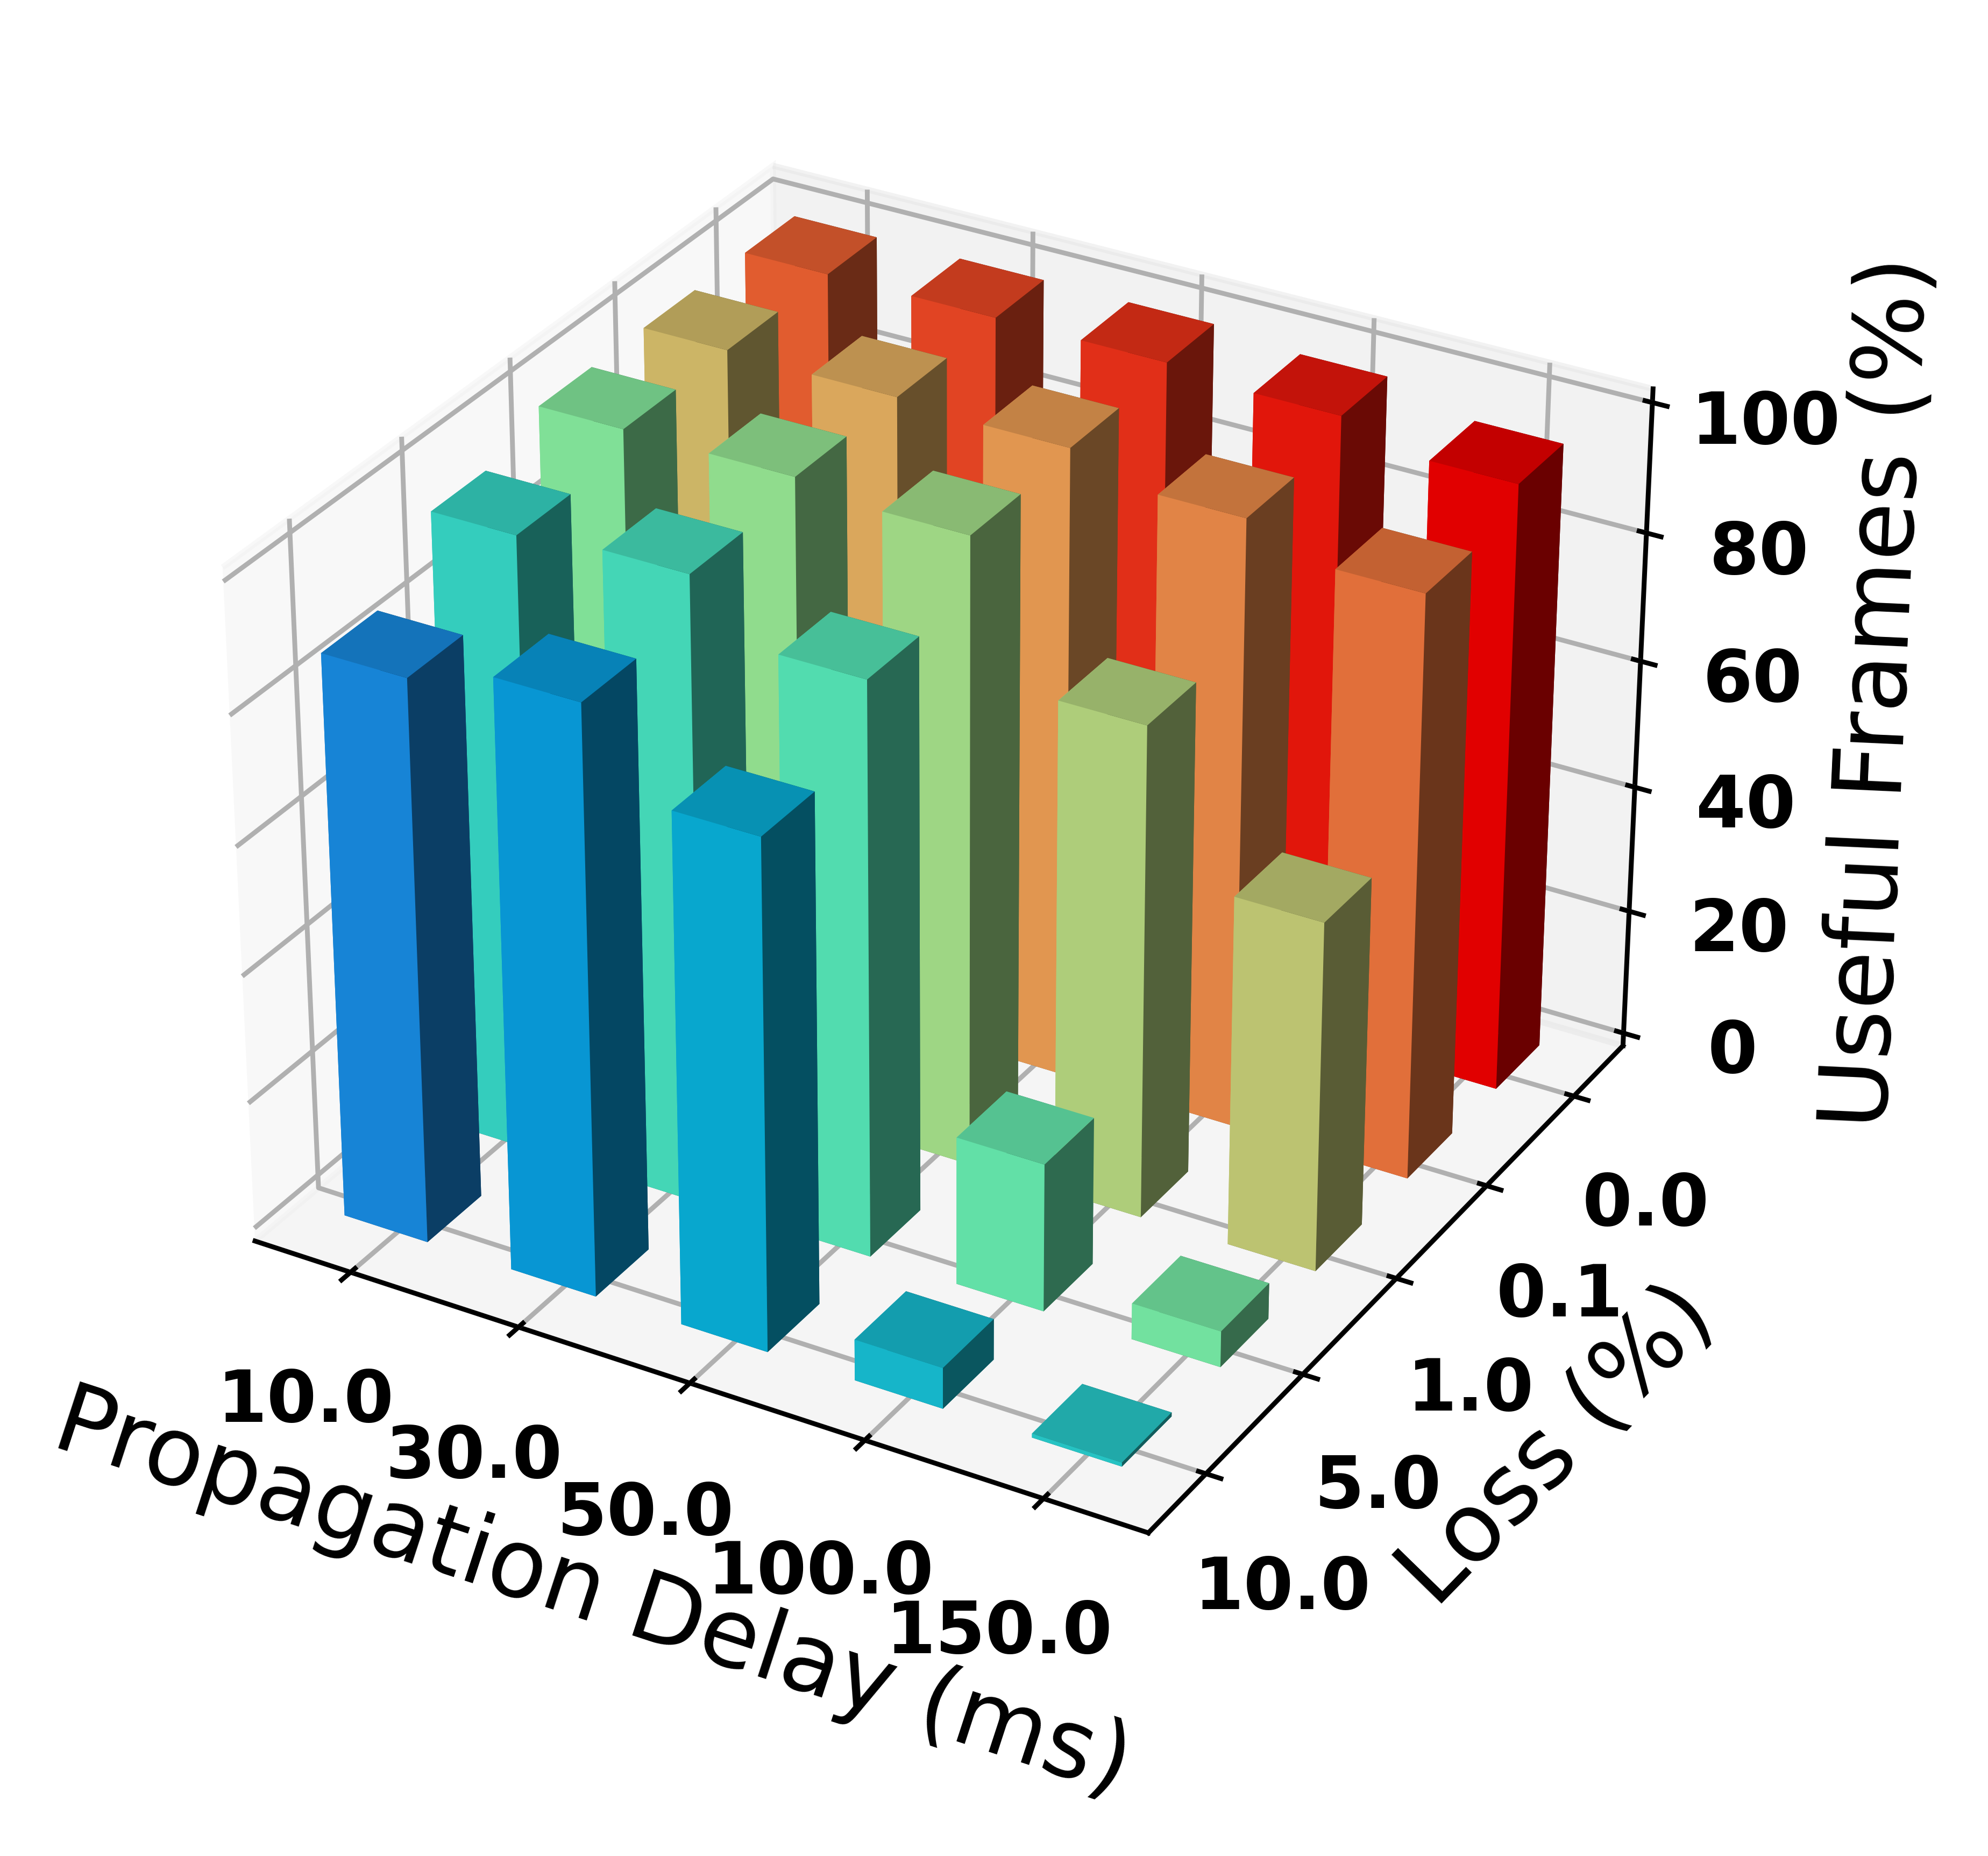
\includegraphics[width=\textwidth]{Frame_Usefulness_Ratio/TCP/AVG_Frame_Usefulness-168.png}
      \caption{TCP: Useful Frames}
      \label{fig:TCP_bar-168}
  \end{subfigure}
  \hfill
  \begin{subfigure}[b]{0.25\textwidth}
      \centering
      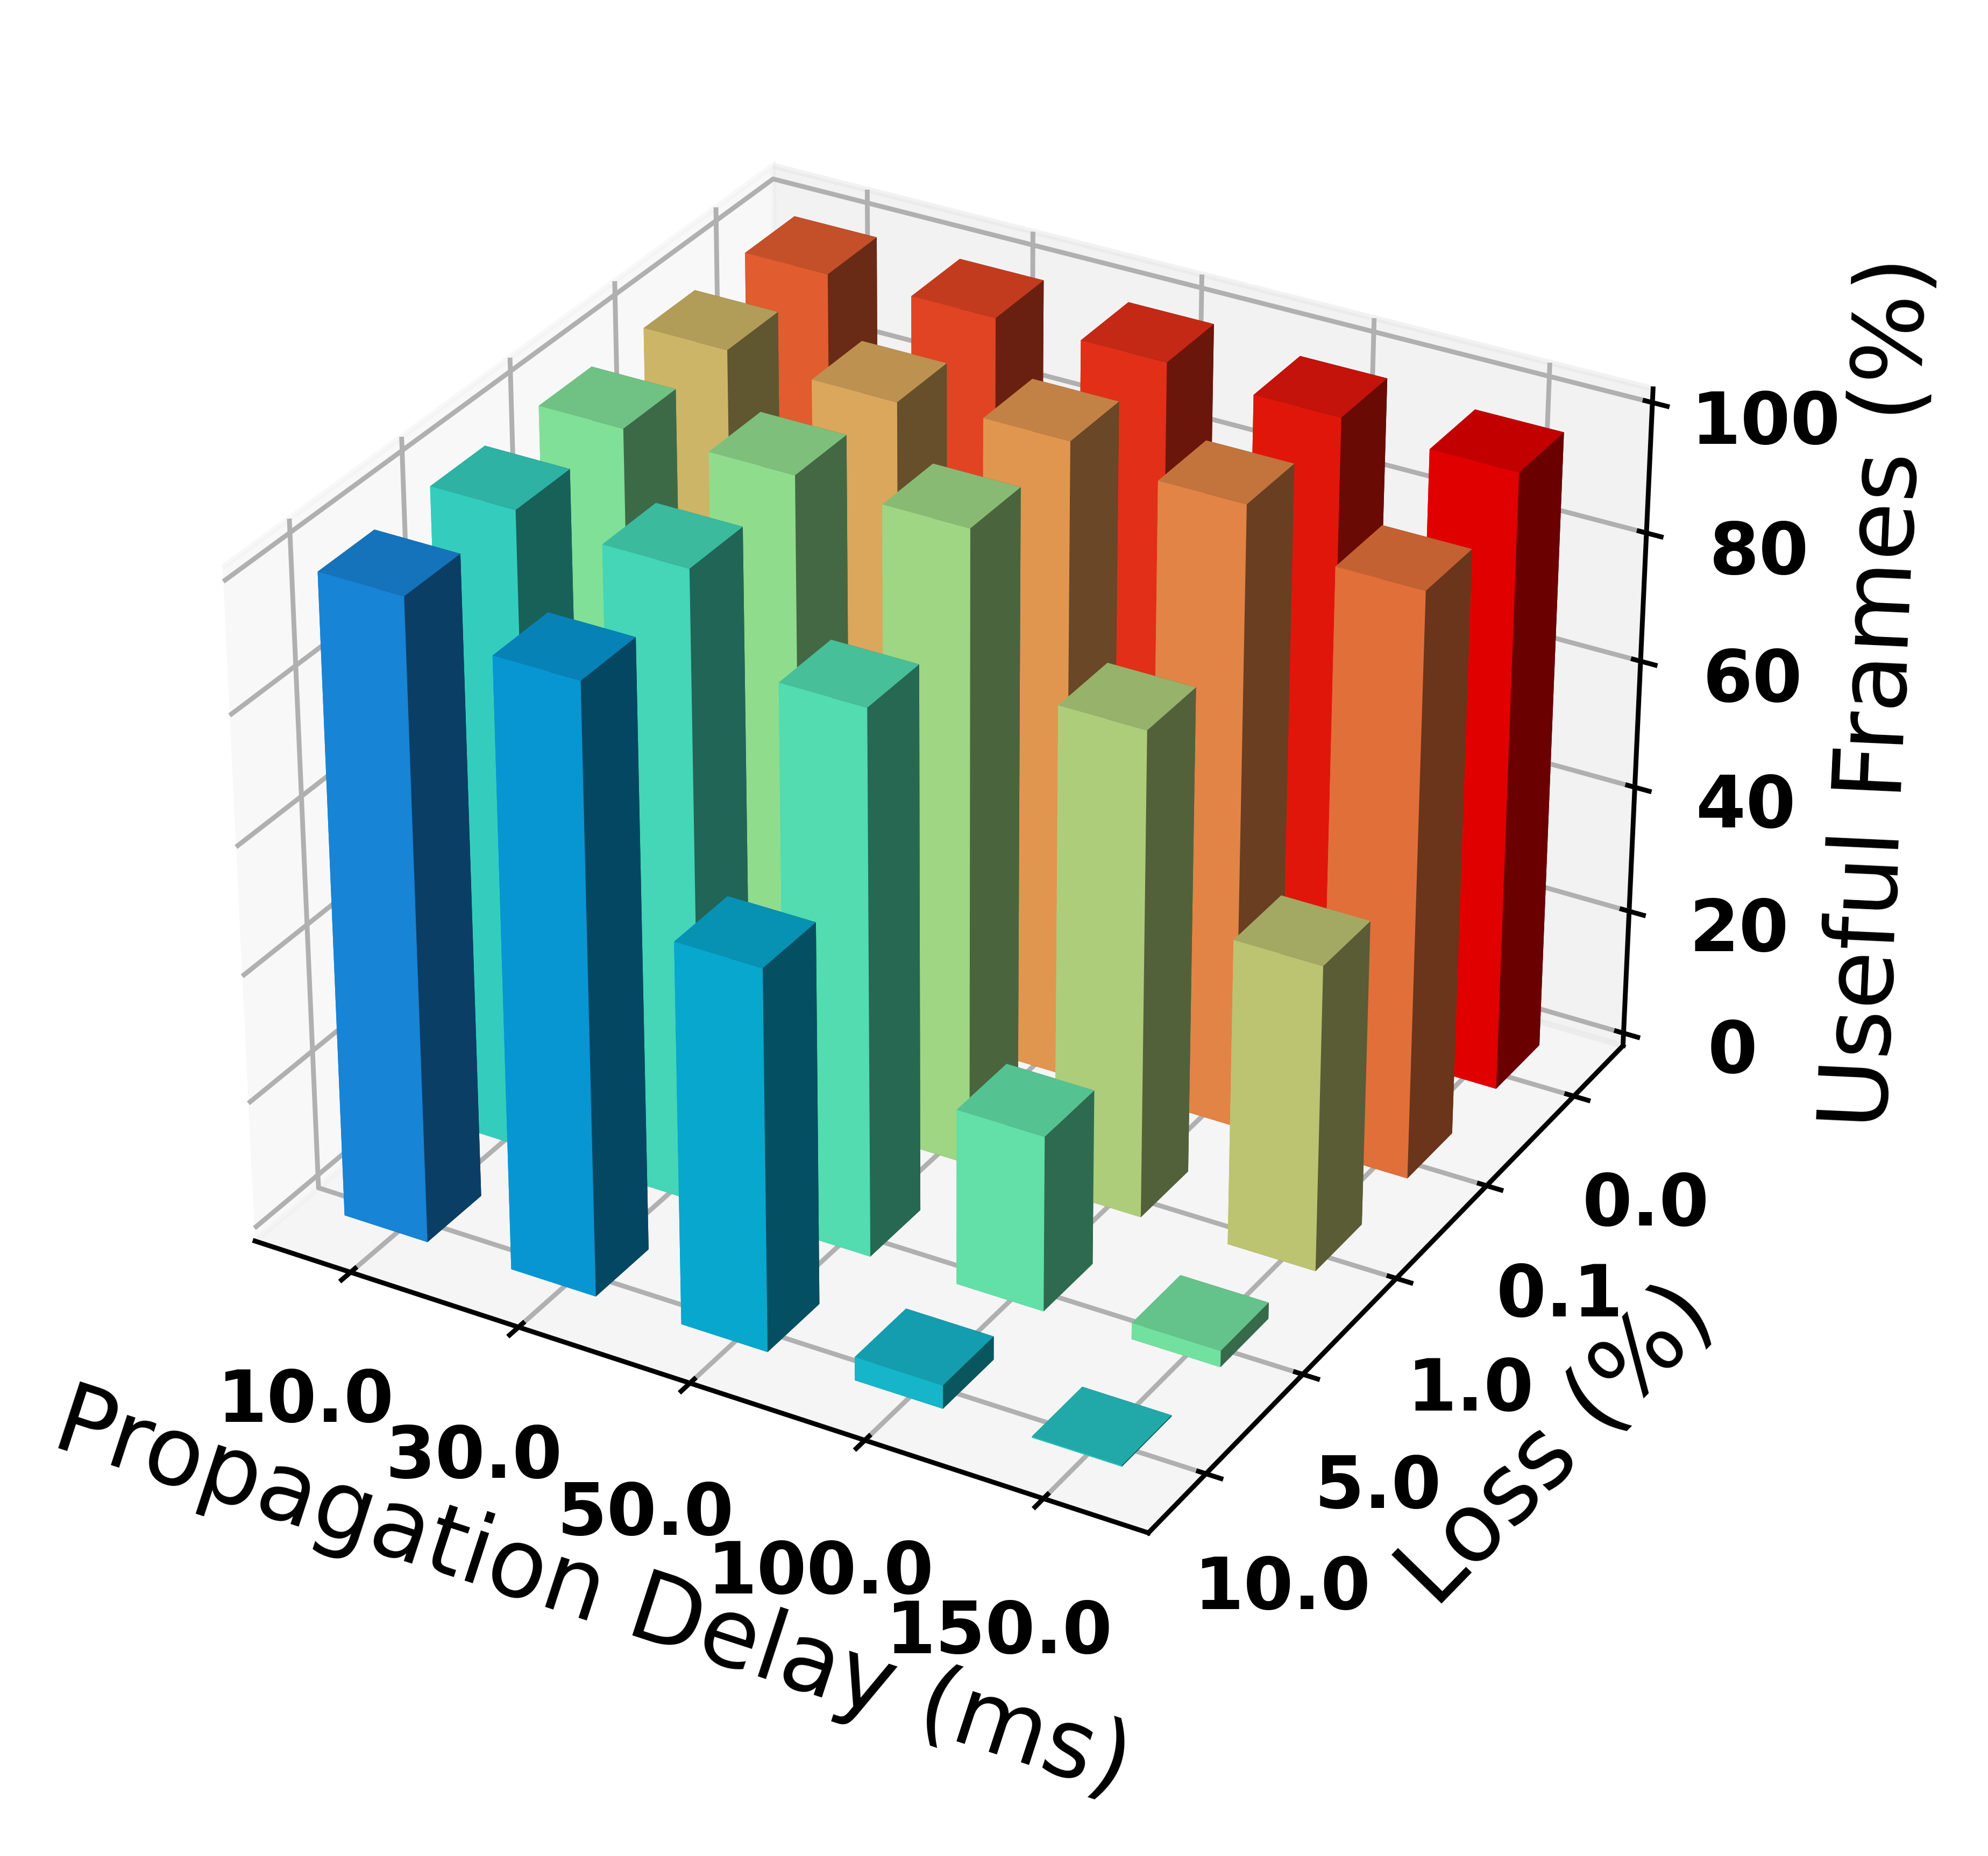
\includegraphics[width=\textwidth]{Frame_Usefulness_Ratio/QUIC_SS/AVG_Frame_Usefulness-168.png}
      \caption{QUIC\_SS: Useful Frames}
      \label{fig:SS_bar-168}
  \end{subfigure}
  \hfill
  \begin{subfigure}[b]{0.25\textwidth}
      \centering
      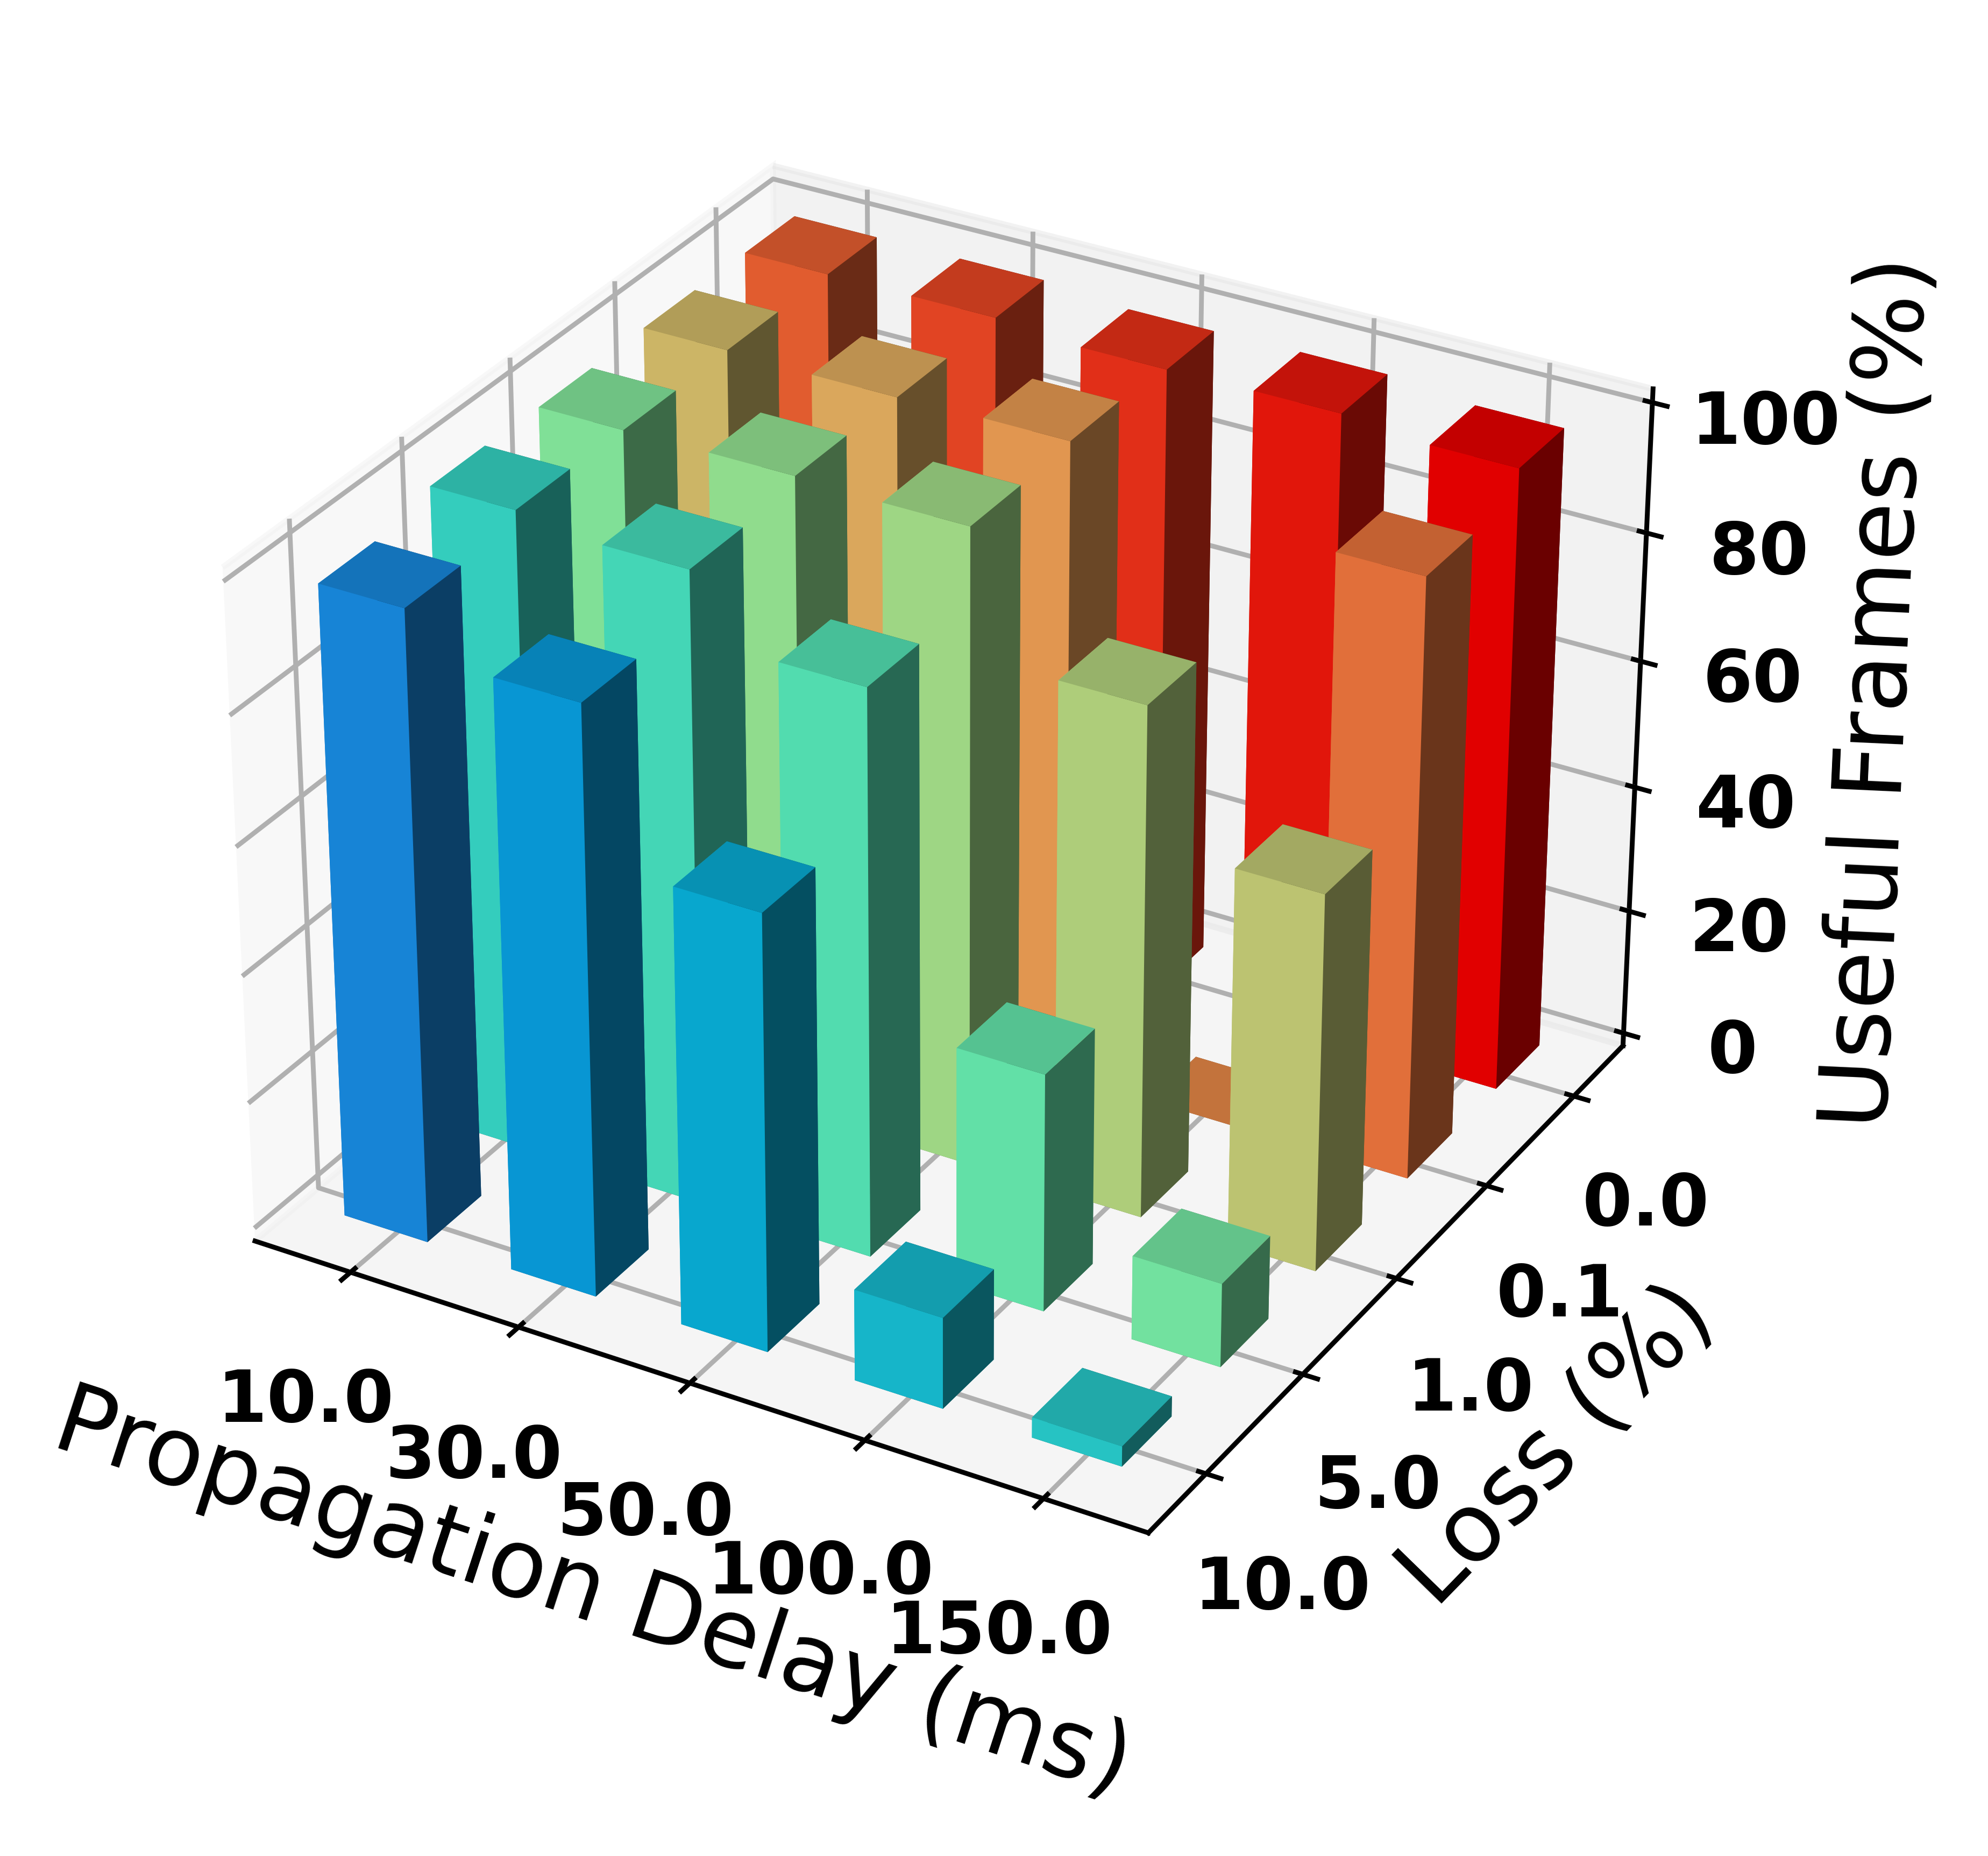
\includegraphics[width=\textwidth]{Frame_Usefulness_Ratio/QUIC_GOP/AVG_Frame_Usefulness-168.png}
      \caption{QUIC\_GOP: Useful Frames}
      \label{fig:GOP_bar-168}
  \end{subfigure}
  \begin{subfigure}[b]{0.25\textwidth}
      \centering
      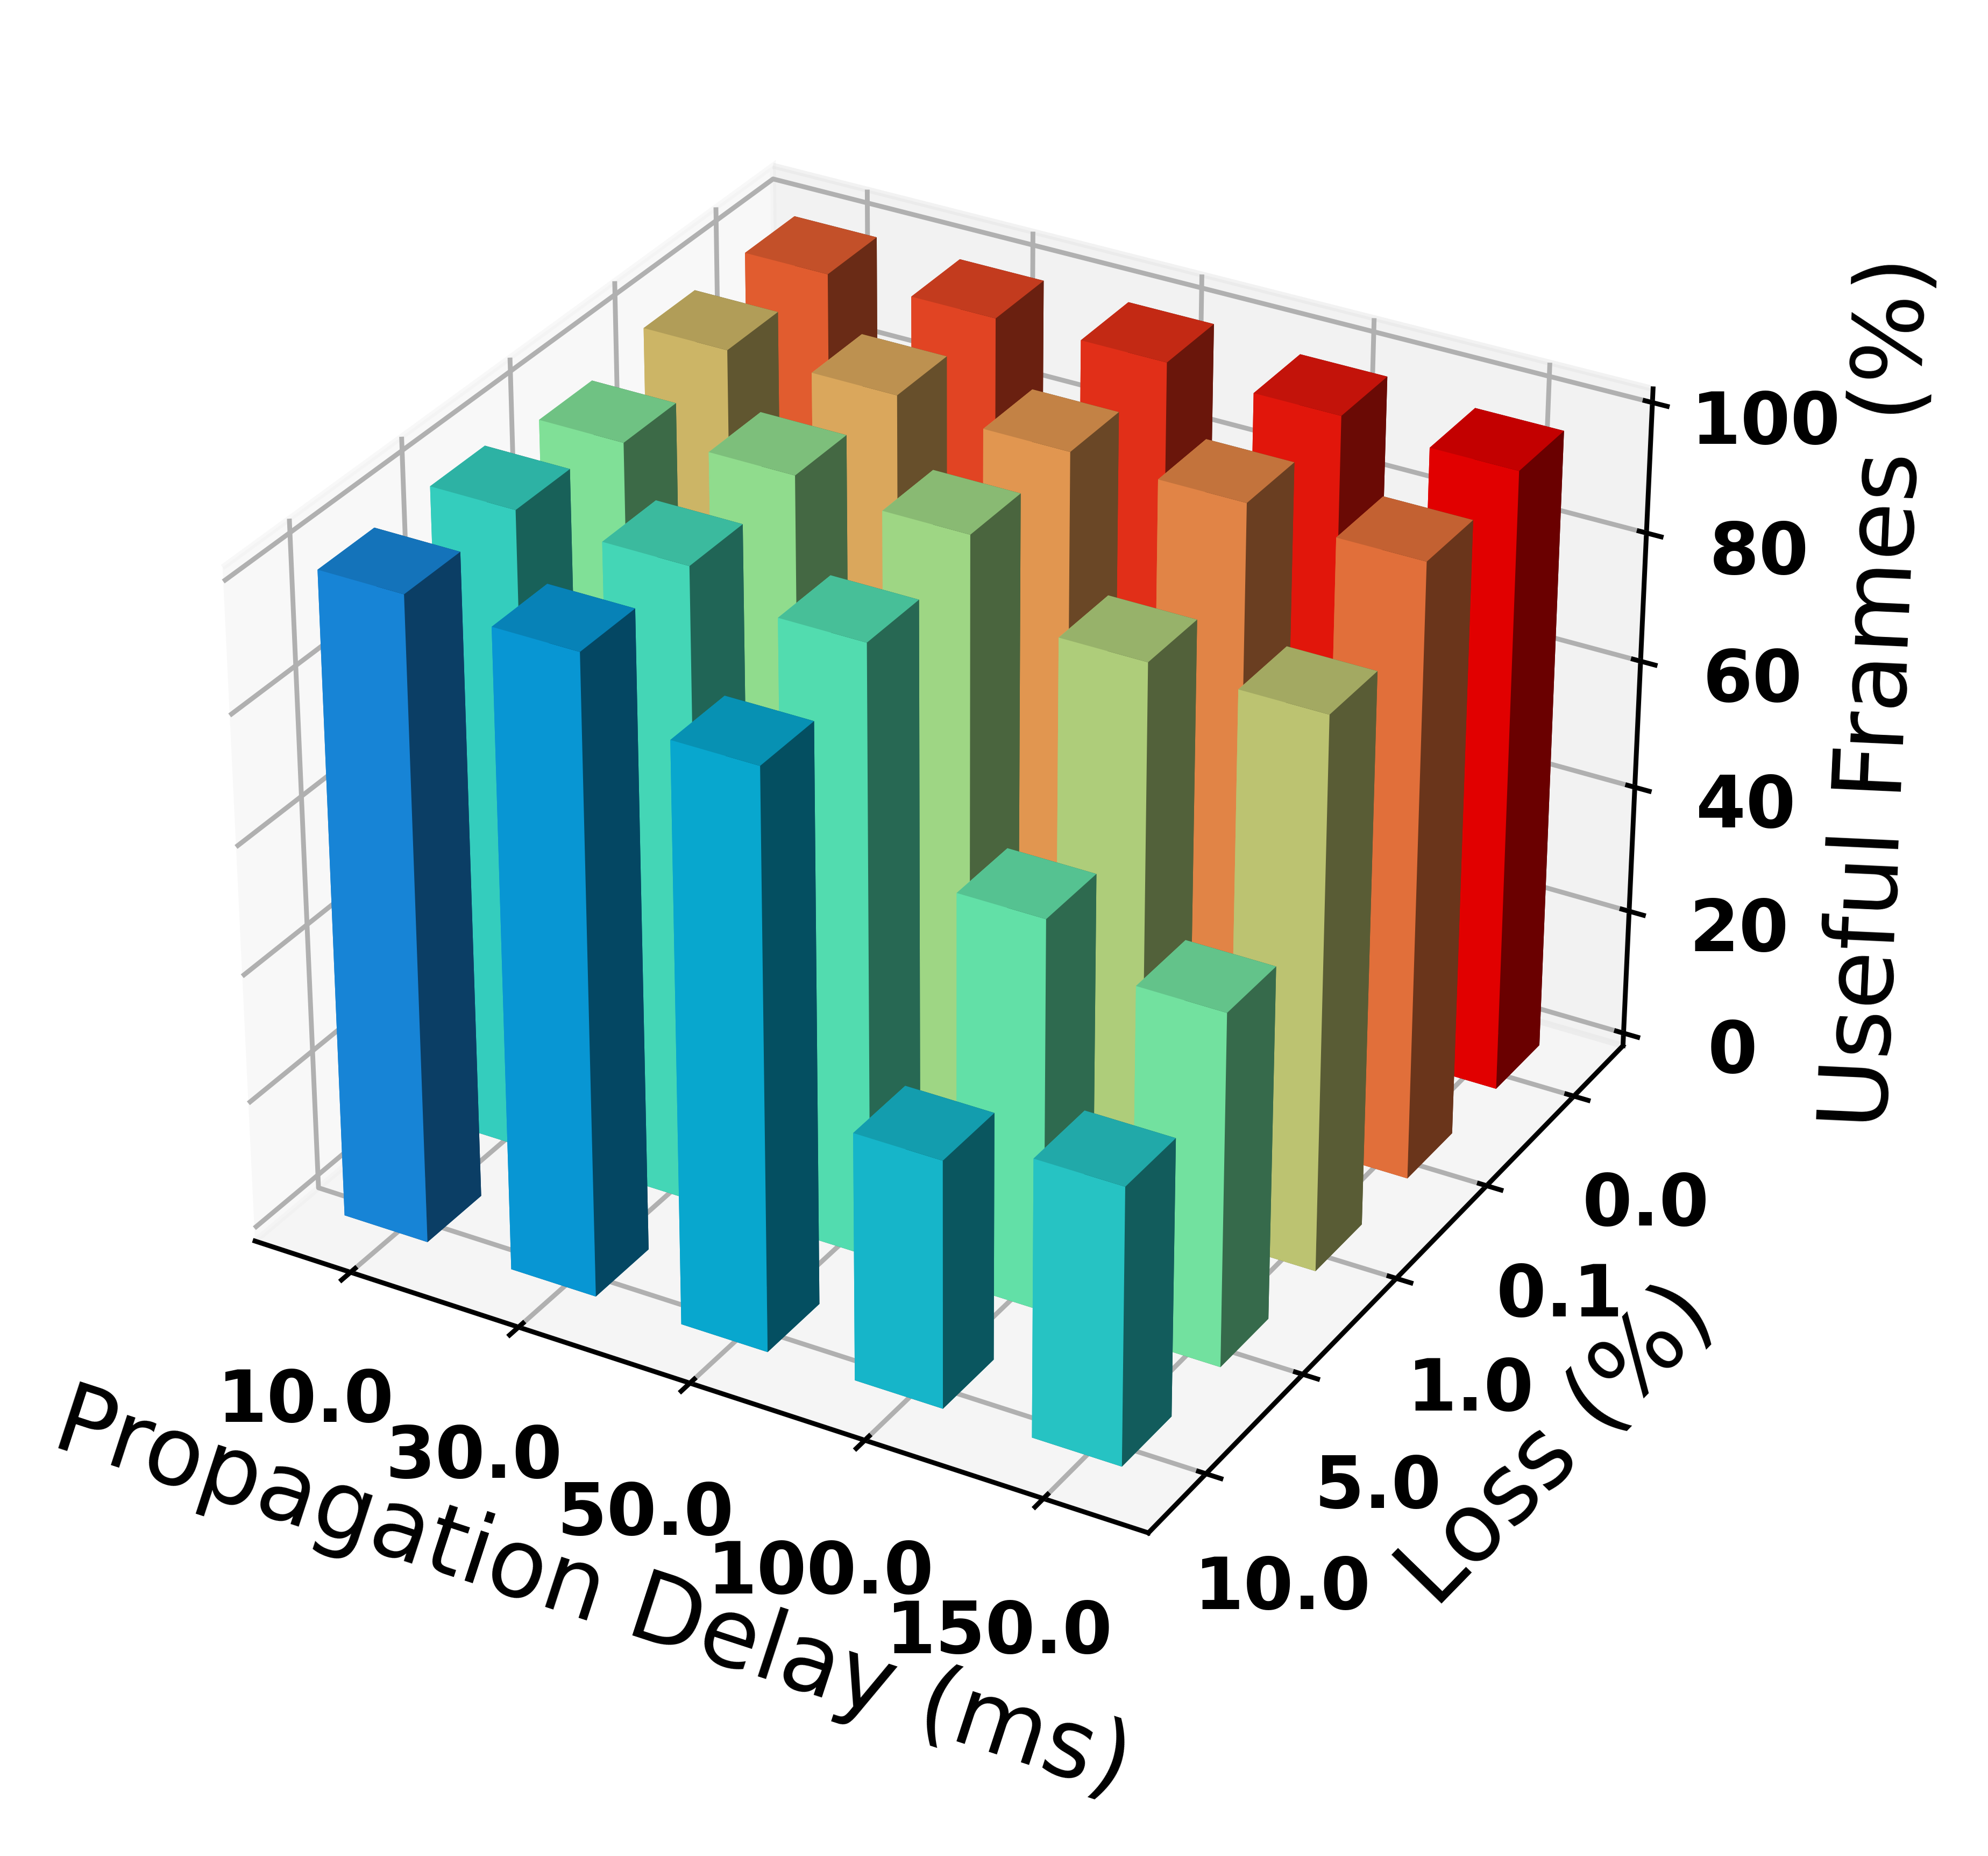
\includegraphics[width=\textwidth]{Frame_Usefulness_Ratio/QUIC_FPS/AVG_Frame_Usefulness-168.png}
      \caption{QUIC\_FPS: Useful Frames}
      \label{fig:FPS_bar-168}
  \end{subfigure}
  \hfill
  \begin{subfigure}[b]{0.25\textwidth}
      \centering
      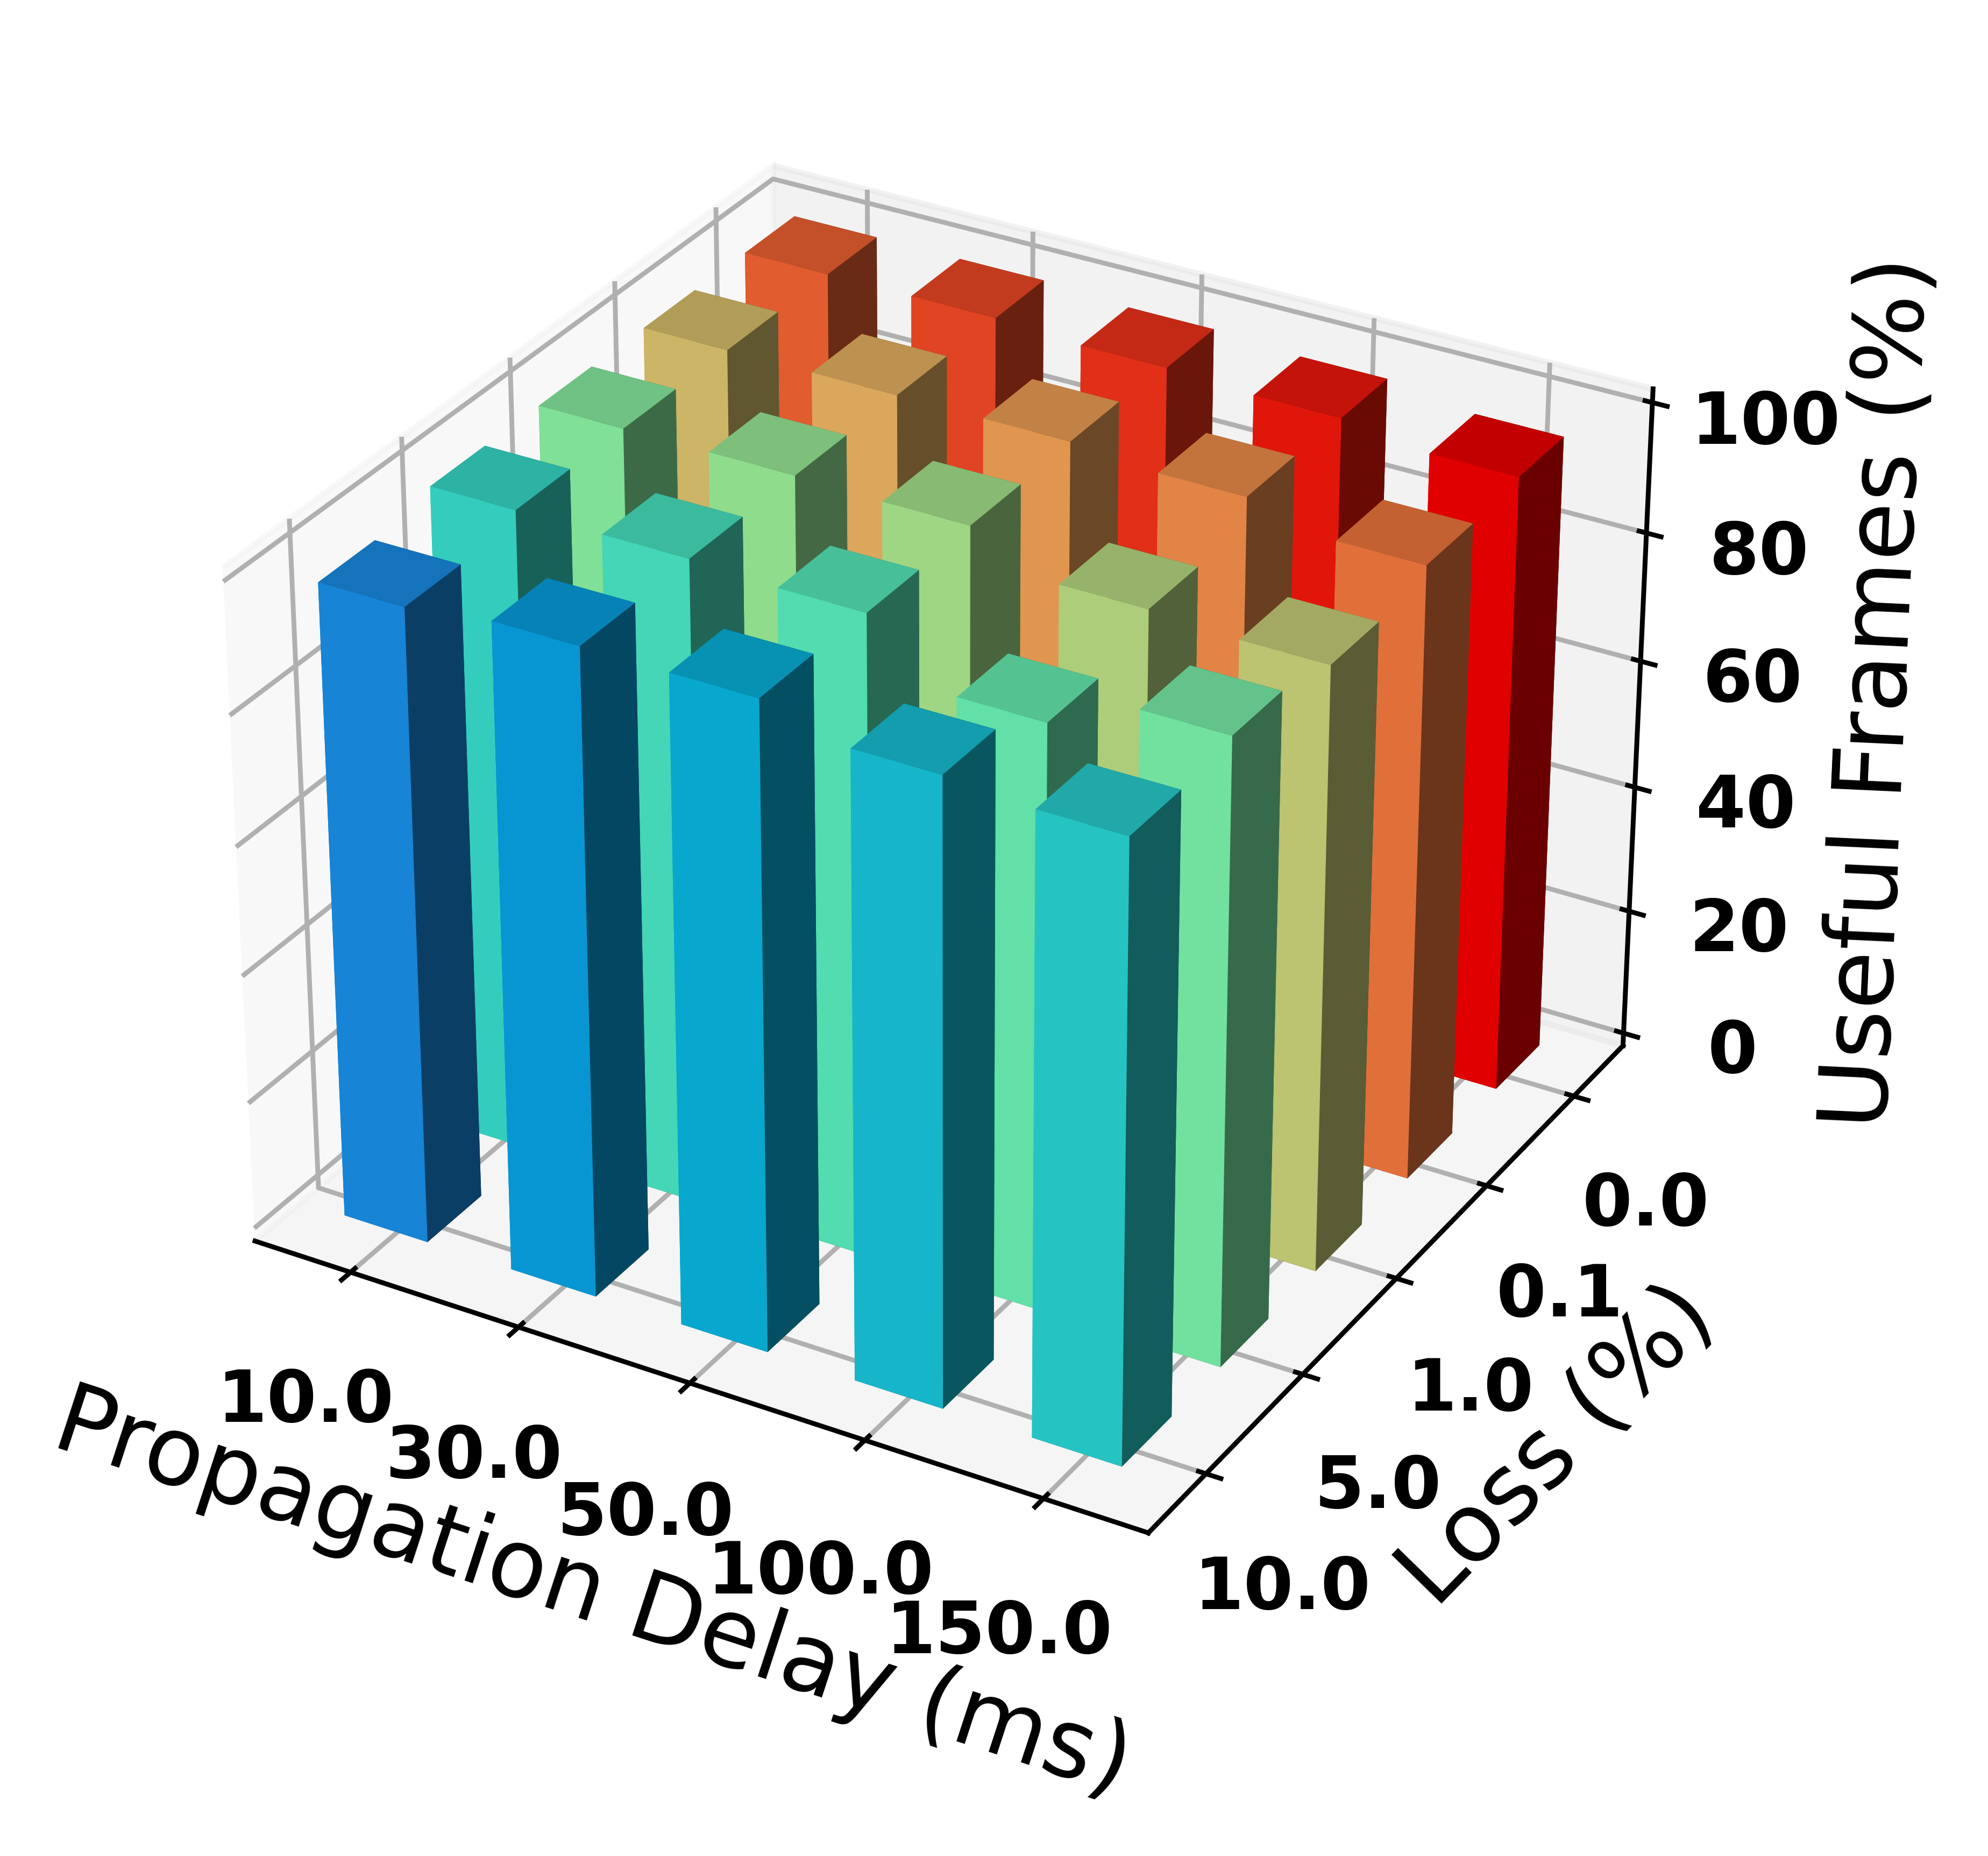
\includegraphics[width=\textwidth]{Frame_Usefulness_Ratio/QUIC_PPS/AVG_Frame_Usefulness-168.png}
      \caption{QUIC\_PPS: Useful Frames}
      \label{fig:PPS_bar-168}
  \end{subfigure}
  \hfill
  \begin{subfigure}[b]{0.25\textwidth}
      \centering
      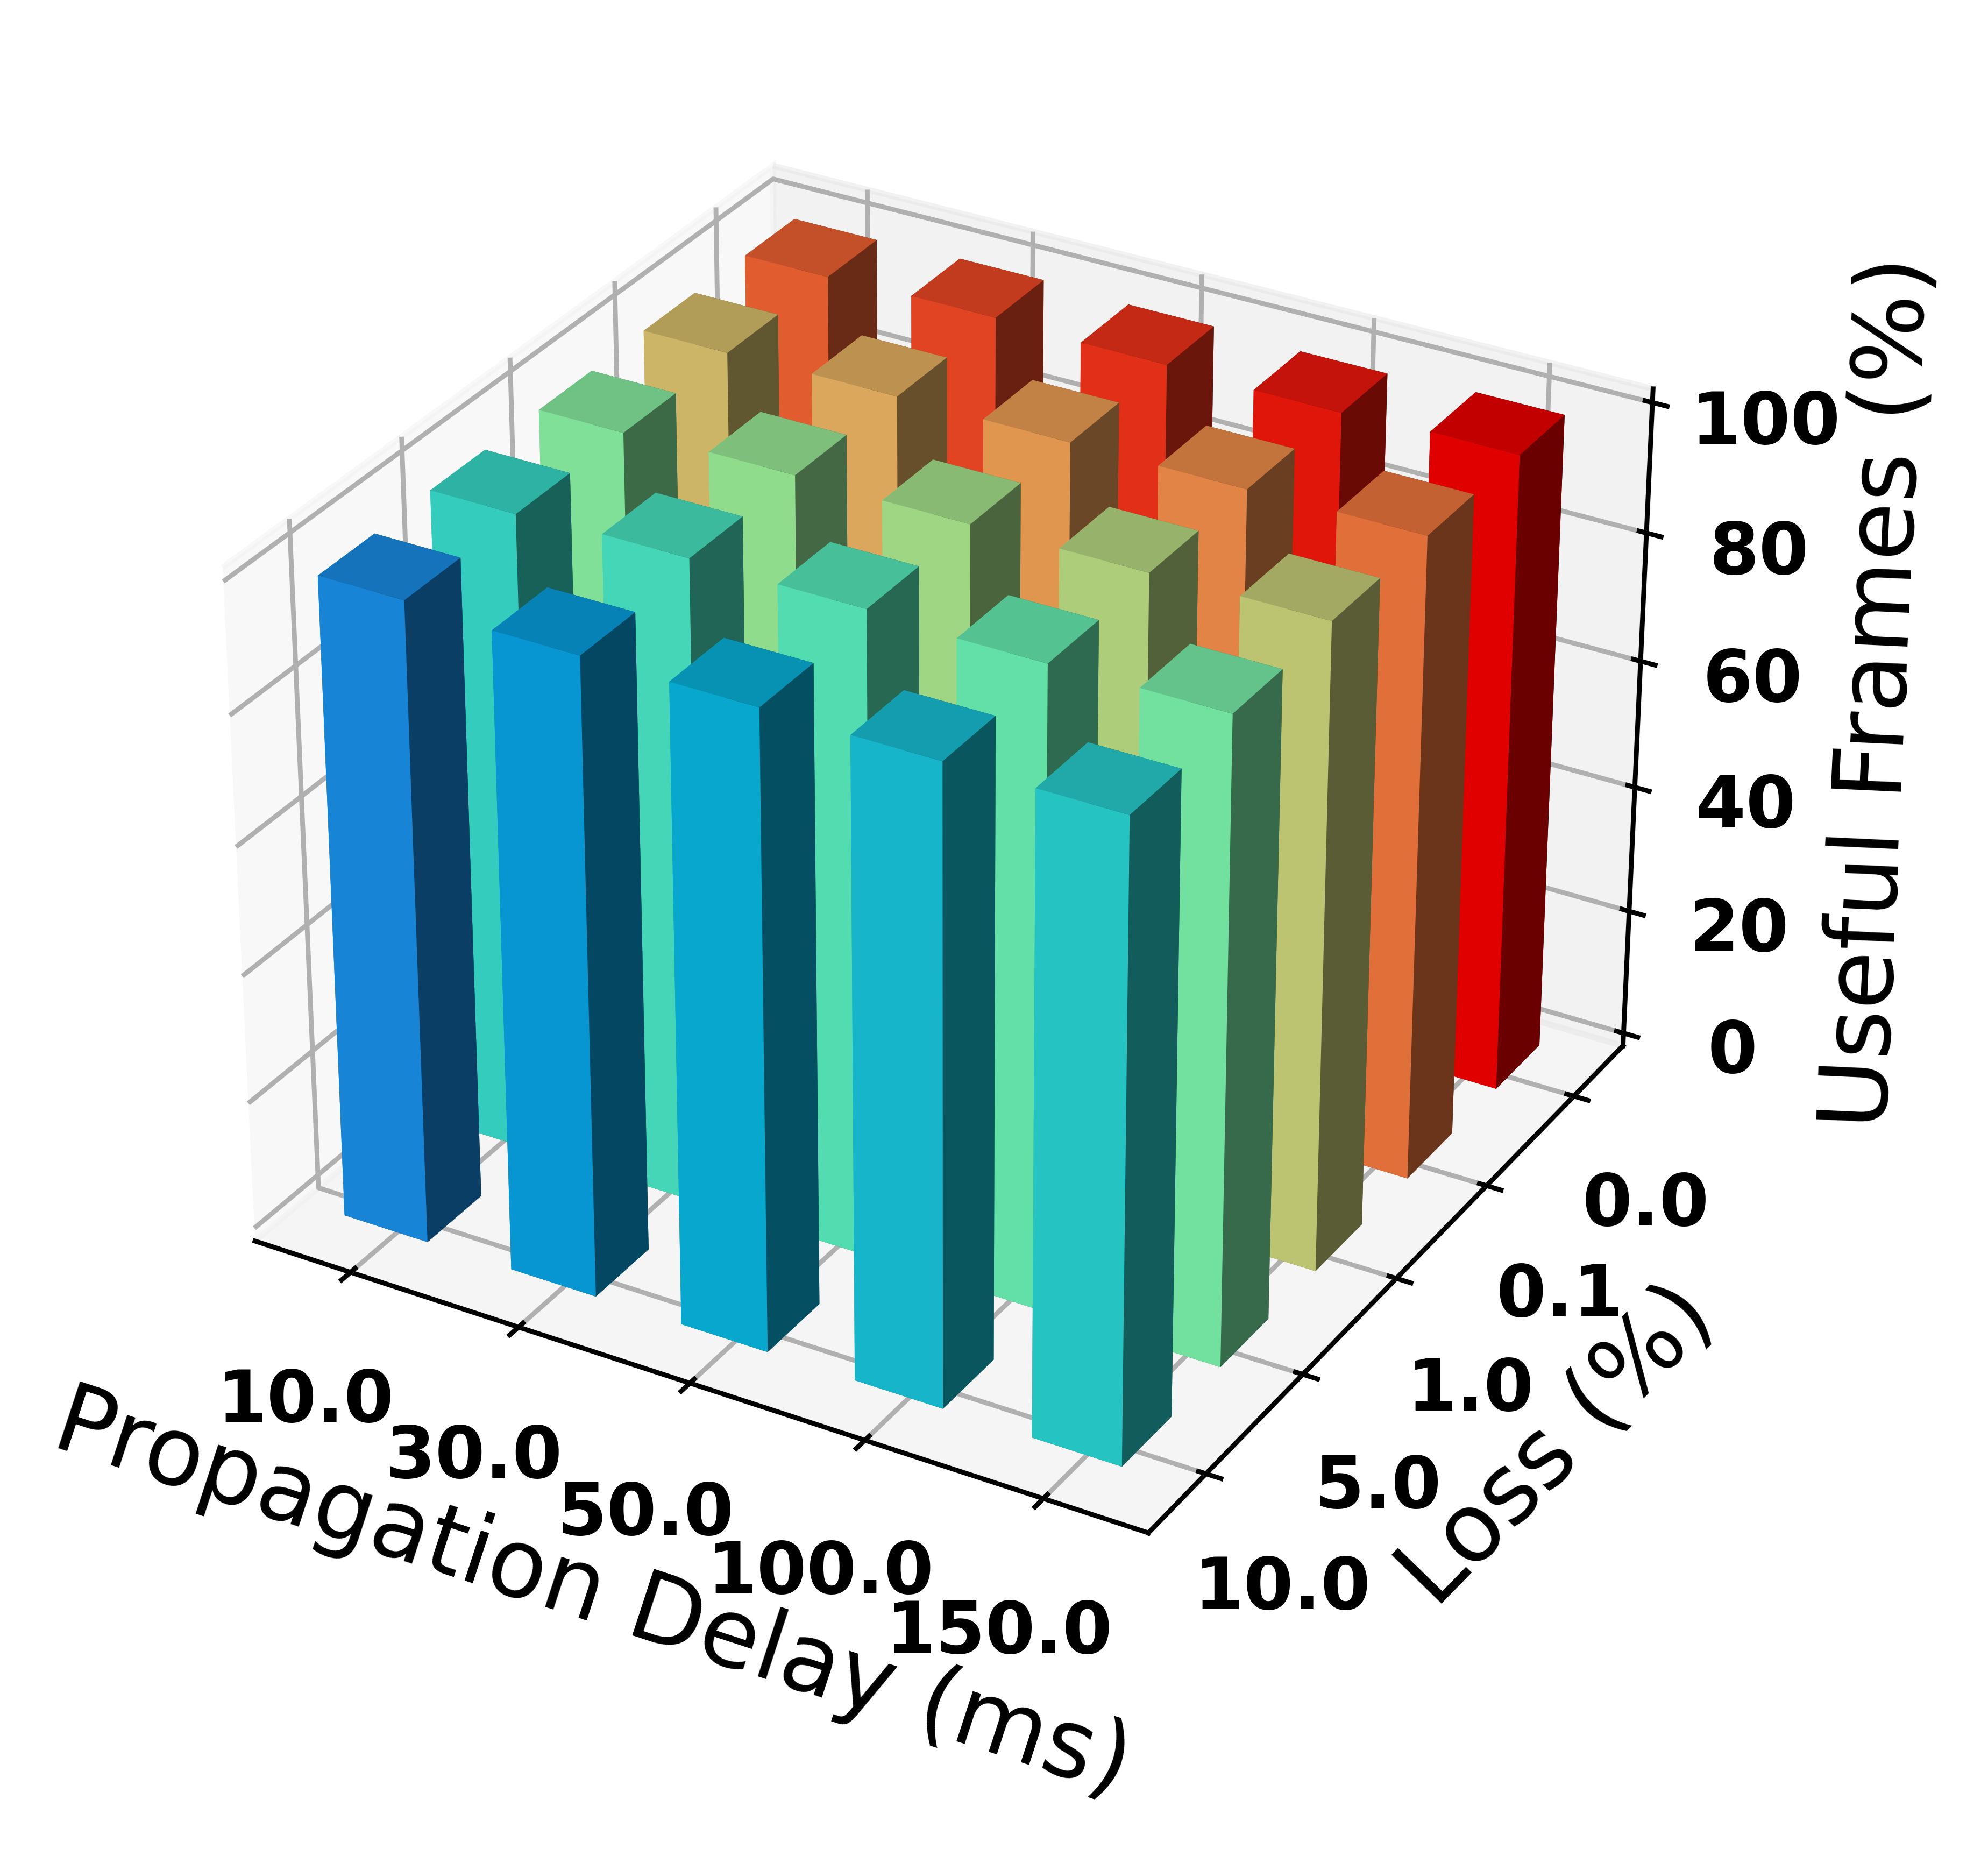
\includegraphics[width=\textwidth]{Frame_Usefulness_Ratio/UDP/AVG_Frame_Usefulness-168.png}
      \caption{UDP: Useful Frames}
      \label{fig:UDP_bar-168}
  \end{subfigure}
     \vspace{0.1cm}
     \centering
     \captionsetup{justification=centering, margin={1.5cm,0cm}}
     \caption{3d bar plots showing the percentage of useful frames delivered by each implementation at different levels of loss and propagation delay. The receive buffer size for these tests was 168ms.}
     \label{fig: 168-bar}
\end{figure*}


\noindent The most important aspect of real-time video transport is the timely delivery of frames to the application. GStreamer's H264 decoder was used to determine if a frame could be considered useful. If enough of a frame is delivered to the decoder before its playback deadline, the decoder will report that it successfully decoded the frame and that there was no corruption. Additionally, for a given frame to be considered useful by the decoder, any frames it depends upon must be delivered beforehand. To compare each implementation, the percentage of useful frames delivered to the decoder was calculated and averaged across 5 iterations of each test scenario.
\\\\
Taking into account the results of the HOL blocking analysis, it was expected that, for QUIC\_SS, QUIC\_GOP, \newline QUIC\_FPS and TCP, the percentage of useful frames would drop with both increasing loss and increasing propagation delay. TCP and QUIC\_SS were expected to perform the worst due to HOL blocking, with QUIC\_GOP expected to perform slightly better and QUIC\_FPS expected to perform significantly better due to differing levels of HOL blocking mitigation. \newline QUIC\_PPS and UDP were expected to perform the best at high latency, high loss scenarios, as they do not experience any HOL blocking. 
\\\\
Additionally, it was expected that the QUIC and TCP implementations would be unlikely to achieve 100\% useful frame delivery, as the sending delay injected by BBR would have an impact even on lossless links. Finally, as UDP has no ability to retransmit, it was expected that as loss increases, UDP's useful frame percentage would fall by an equal amount (e.g. at 10\% loss UDP would deliver 90\% useful frames).
\\\\
Figure \ref{fig: 42-bar} contains 3d bar plots for each implementation. Each plot shows the percentage of useful frames delivered for each loss and propagation delay tested. The receive buffer delay was 42ms for the scenarios represented by \ref{fig: 42-bar}. This provides a very short window for retransmission and has the lowest tolerance for delayed packets out of the four buffer delays used during evaluation. On the next page, a similar set of bar plots is shown in figure \ref{fig: 168-bar}.  Figure \ref{fig: 168-bar} provides the useful frame ratios when the buffer delay is 168ms, allowing significant time for retransmission.
\\\\
Surprisingly, despite its lack of any retransmission mechanisms, UDP performed well across the board. In the worst-case scenario, where 10\% of all packets would be lost in transit, one would expect that UDP would fail to deliver around 10\% of frames with sufficient data to be decoded. However, UDP successfully delivered between 97\%and 99\% of frames with sufficient data to be decoded. This demonstrates the power of redundancy; For the 720p Big Buck Bunny video used during testing, each P-frame is typically split into 9 to 11 NAL units. At 10\% loss and below, it is reasonable to expect that only 1 NAL unit will be lost per frame.  As the other NAL units carry redundant data, the decoder is able to recover. When multiple NAL units are impacted by packet loss, insufficient data is provided to the decoder, and the frame is not useful. This scenario is rare, only occurring on high loss tests (5\%, 10\%). Additionally, UDP gets no benefit from a larger buffer delay on the client-side, allowing the delivery of data with as little latency as possible.
\\\\
As expected, as loss is introduced and delay is increased, the impact of HOL blocking quickly becomes evident. QUIC\_SS and TCP's useful frame delivery ratio quickly drops, eventually into single figures at higher propagation delay and loss rates. This is true even with a large receive-side buffer delay, as shown in figures \ref{fig:TCP_bar-168} and \ref{fig:SS_bar-168}. QUIC\_GOP does manage to outperform QUIC\_SS and TCP, demonstrating that even a small reduction in the amount of HOL blocking can make a big difference. However, QUIC\_GOP does become essentially useless for low-latency streaming on lossy networks once the delay surpasses 50ms. QUIC\_FPS significantly outperforms TCP, QUIC\_SS, and QUIC\_GOP on high latency, lossy links. QUIC\_FPS manages to achieve a useful frame ratio of above 70\% at 150ms of delay and 1\% loss where the previous implementations had fallen to around 50\%. At 150ms delay and 5\% loss, it still achieves above 50\% useful frame delivery. These values still pale in comparison to the frame latencies achieved by UDP.
\\\\
By eliminating HOL blocking, QUIC\_PPS vastly outperforms TCP and the other QUIC implementations. Even at the highest delay and loss tested, the useful frame ratio exceeds 90\%. In some low-delay high-loss scenarios, \newline QUIC\_PPS is even able to outperform UDP, suggesting that retransmissions can be useful in these cases. However, these may just be outliers, as in the majority of scenarios, \newline QUIC\_PPS still suffers from the consequences of congestion control. While this issue exists, UDP will outperform congestion-controlled protocols even when HOL blocking is completely eliminated.

\section{Related Work} \label{Related Work}

\noindent QUIC\_PPS is not the first attempt at eliminating HOL blocking within reliable streams. In 2016, McQuistin et al. presented a modification of the TCP protocol: TCP Hollywood\cite{Hollywood}. TCP Hollywood makes three changes to standard TCP. The first is an intermediary layer which provides a messaging abstraction on top of the TCP stream. The second is referred to as 'inconsistent retransmission'. Metadata is provided alongside messages to be sent. When a message is lost, the timing and dependency data are examined. If based on the estimated RTT, a message can be retransmitted in time to be useful, or if a later message is dependent on the lost message, then the message is retransmitted. Otherwise, the content of the retransmission is replaced with new data. The third change eliminates HOL blocking by permitting out of order delivery. The TCP kernel will provide data to the intermediary layer as soon as it arrives, and the intermediary layer will reconstruct messages to be passed to the application. By preventing unnecessary retransmissions and HOL blocking, TCP Hollywood successfully improved upon the performance of standard TCP when used for real-time multimedia applications. While TCP Hollywood is certainly effective, its deployability suffers due to the kernel-based nature of TCP. Extensions and modifications made to TCP have, in the past, taken up to a decade to deploy\cite{Fukuda}. As QUIC is typically implemented in userspace, the methods presented in this paper suffer no such deployability issues while achieving similar results.
\\\\
Palmer et al. present a similar but less sophisticated approach when compared to TCP Hollywood, ClipStream, created through modifications to QUIC in their 2018 paper\cite{ClipStream}. The message abstraction layer is replaced by QUIC streams, each of which carries a single video frame. The end of each stream indicates the complete delivery of a frame. However, rather than selectively retransmitting frames based on an estimated playback deadline, it is assumed that the loss of P-frames is insignificant, and the payload of packets scheduled for retransmission is replaced by new data. As it is possible that these frames could arrive before the playback deadline, it seems careless to abandon retransmission without any attempt to determine whether or not they will arrive too late. Additionally, while ClipStream improves upon the performance of standard QUIC and TCP, no comparison is made to a QUIC implementation that simply utilises a reliable stream for each frame. It was unclear from the results whether or not the removal of HOL blocking by sending each frame in a separate stream is the main cause of improvement, rather than "opportunistic retransmission", as the paper suggests. The findings of this paper confirm the effectiveness of eliminating HOL blocking between frames and demonstrates that going further and eliminating HOL blocking between RTP packets can further reduce delays.
\\\\
In another attempt to improve the performance of real-time multimedia streaming, Vivian Band presented her own modifications to QUIC\cite{QUICSilver}. Band's implementation, QUICsilver, took a different approach to avoid the HOL blocking problem than Palmer's ClipStream. QUICsilver uses a single stream, and, like TCP Hollywood, the client and server have an awareness of the playback deadline for each frame. On the server-side, if the server determines that a packet will not arrive in time to be useful, it is removed from the retransmission buffer. On the client-side, if a packet has not arrived before its playback deadline, it is considered stale, and the stream read offset is increased so that subsequent packets can be provided to the application. The deadline awareness utilised by QUICsilver is, in theory, effective at eliminating the HOL blocking issue. However, in order for the client to increase the read offset by the correct amount, QUICsilver requires prior knowledge of the size of each frame. Sending control data at the start of a connection (frame size, I-frame interval, etc.) may make this possible for encoders that produce consistently sized I-frame and P-frame. Many encoders do not produce consistently sized frames, so QUICsilver may have limited usability in practice. This paper presents a different approach for eliminating HOL blocking without any foreknowledge required by the client.


\section{Conclusions} \label{Conclusions}

\noindent This paper presents an evaluation of three different methods for reducing/eliminating HOL blocking via the use of QUIC streams: QUIC\_GOP eliminates HOL blocking between GOPs; QUIC\_FPS eliminates HOL blocking between frames; QUIC\_PPS eliminates HOL blocking entirely by using a stream for every RTP packet sent.
\\\\
The first of the two questions this paper sought to answer was: \textit{'Can QUIC provide a reduced latency compared to TCP when used to transport real-time video, without sacrificing video quality?'}
\\\\
The results show that each implementation outperforms TCP and single-stream when delivering real-time video data under strict latency bounds. While QUIC\_GOP and QUIC\_FPS are capable of reducing latency compared to TCP, the HOL blocking that still exists in the implementation results in a low percentage of frames being delivered to the application before the playback deadline on lossy networks. Due to this, these implementations would not be practical for real-time video streaming. QUIC\_PPS, on the other hand, while not perfect, delivers a high percentage of frames with sufficient data to be decoded before the playback deadline. Therefore, QUIC\_PPS provides an effective replacement for TCP for the purposes of low-latency streaming.
\\\\
The second question this paper sought to answer was: \textit{'Can QUIC deliver better quality real-time video than UDP, while operating within the strict latency bounds of interactive media?'}
\\\\
While QUIC\_PPS can deliver a high percentage of real-time video data under strict latency bounds, it does not surpass UDP. Although QUIC\_PPS is capable of retransmitting lost packets, the delays imposed by congestion control outweigh the benefit of retransmission. While UDP does not make any attempt to retransmit lost packets, the redundancy present in NAL units allows the decoder to recover from small amounts of data loss with frames. As a result, for real-time multimedia with strict latency bounds, UDP remains the superior choice for the time being.
\\\\
Finally, the results of the research also include GStreamer element plugins that integrate the QUIC transport protocol into GStreamer. At the time of writing, no other QUIC plugins for GStreamer are available. The source code for the plugins can be found at https://github.com/mwalker2299/QUIC-GStreamer-Integration.

\section{Future Work} \label{Future Work}

\noindent Producing the GStreamer elements and pipelines used for evaluation required significant effort. This left less time for testing, and due to the time required to run real-time multimedia tests, a number of test scenarios were cut. In the end, a single bandwidth of 1 Gbps was used during testing. This bandwidth was significantly higher than the bitrate of the video stream, and so the router buffers would never fill. Future experiments could investigate the behaviour of QUIC\_PPS and UDP when working with a bandwidth closer to the bitrate of the video stream. Suppose, without any congestion control, UDP sends too fast and fills the router buffer at the bottleneck link. In that case, multiple consecutive packets may be lost due to congestion, leading to an incomplete frame. Additionally, as the router buffer fills, the RTT will increase, leading to an increased delay in the arrival of UDP packets. QUIC\_PPS would not experience this, as BBR would send at a rate that fully utilises the bottleneck link without filling the buffer. This provides a potential avenue for future work.
\\\\
Additionally, the main cause of delay in QUIC\_PPS was the BBR congestion control algorithm used. The results show that BBR has an impact on delay, even in lossless scenarios. Other congestion control algorithms such as CUBIC would not have the same impact on lossless links. Alternatively, TCP Vegas is another congestion control algorithm that, like BBR, does not use loss as an indicator of congestion. Exploring the existing algorithms and providing mappings to QUIC could potentially reveal a method for eliminating the congestion control based delay that prevented QUIC\_PPS from surpassing UDP.
\\\\
QUIC\_GOP, QUIC\_FPS and QUIC\_PPS are all designed to work with a single video stream. In practice, audio streams will be sent simultaneously. As they exist now, the implementations evaluated in this paper would have no way of differentiating between streams carrying audio data and streams carrying video data. To improve this, a control stream could be added to indicate which streams contain audio data and video data, allowing the client to handle each as appropriate.
\\\\
Finally, to avoid delays due to flow control limits, the QUIC-GStreamer elements had to have their initial values raised so that the flow control limits would not be reached. The initial values required were found through experimentation, but this would not be possible in practice. Future work could develop an algorithm for raising flow control limits at the client-side explicitly designed to combat the bursty nature of real-time video traffic.


\section{Acknowledgments}

\noindent I would like to thank Dr Colin Perkins, both as an advisor and as a lecturer, for his enthusiastic advice and wisdom throughout this project. I knew I could always turn to him for new ideas or potential solutions. I would also like to thank my loving mother, grandfather and grandmother for all their kind words and support during my final year.

\bibliographystyle{abbrv}
\bibliography{bibfile}


\end{document}